\documentclass[cn,blue,12pt]{elegantbook}
\input {d:/tex/preamble}

\excludecomment{note}
\excludecomment{solution}
\renewcommand \tkt[1]{{\CJKunderline[hidden=true, skip=true, thickness=1pt]{#1}}}

\begin{document}

\tableofcontents

\mainmatter

\part{数与式}%
\label{prt:数与式}
\chapter{实数基础概念}%
\label{cha:实数基础概念}

\section{知识要点}%

\begin{zsyd}
\item 实数的分类:\tkt{\(\begin{cases}
            \text{有理数}\begin{cases} \text{整数}\begin{cases} \text{自然数}\begin{cases} \text{正整数}\\ 0\end{cases}\\ \text{负整数}\\ \end{cases}\\ \text{分数}\begin{cases} \text{有限小数}\\ \text{无限循环小数}\\ \end{cases} \end{cases}\\ 
            \text{无理数}
    \end{cases}\)}
\item 无理数:\tkt{不能用两个整数的比表示}的数.也称为\tkt{无限不循环}小数,若将它写成小数形式,小数点之后的数字有\tkt{无限多个},并且\tkt{不会循环}.
    \begin{zsyd}
    \item 常见无理数类型 \tkt{\(\begin{cases} \text{开方开不尽的数:如}\sqrt{2},\sqrt{5},\textbf{注意}\sqrt{4},\sqrt[3]{-8} \text{等是有理数;}\\ \text{化简后含有根号的三角函数值,如}\sin45^\circ,\sin60^\circ,\cos30^\circ,\tan30^\circ;\\ \pi \text{及含}\pi\text{的数:如}2\pi ,\frac{\pi }{2};\\ \text{有规律但不循环的无限小数:如}0.1010010001 \cdots \text{(相邻两个1之间依次多一个0)}. \end{cases} \)}
    \item 【易错警示】 判断一个数是否为无理数, 先要\tkt{化成最简结果}, 然后再判断.如\((\sqrt{2})^2,\, 3.14\)就\tkt{不是}无理数.
    \end{zsyd}
\item 正负数的意义:正负数可以用于表示\tkt{相反意义的量}.如规定``盈(+) '' , 则``亏(-)'', ``胜(+) '' , 则``负(-)''等.
\item 数轴
    \begin{zsyd}
    \item 数轴三要素:\tkt{原点},\tkt{正方向},\tkt{单位长度}\\
            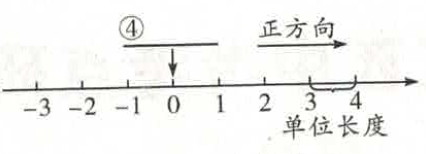
\includegraphics[width=0.8\linewidth]{pic/20200511012.png}
    \item \tkt{实数}与数轴上的点是一一对应的.
    \item 数轴上两点\(a,b\)的距离:\(|a-b|\),数轴上两点的中点:\(\frac{a+b}{2}\)
    \end{zsyd}
\item 相反数
    \begin{zsyd}
    \item 非零实数 \(a\) 的相反数为 \tkt{\(-a\)} ,特别地,\(0\)的相反数为\tkt{\(0\)};
    \item 实数a,b互为相反数\(\iff \) \tkt{\(a+b= 0\)} ;
    \item 互为相反数的两个数表示的点分别位于数轴上原点的\tkt{两侧}, 且到原点的距离\tkt{相等},即互为相反数的两个数在数轴上关于 \tkt{原点} 对称.
    \end{zsyd}
\item 绝对值
    \begin{zsyd}
    \item \(|a|=\)\( \begin{cases} a, & a>0\\ 0, & a=0\\ -a, & a<0 \end{cases} \)
    \item 绝对值具有\tkt{非负}性, 即\(|a|\)\tkt{ \(\ge \)}\(0\);
    \item 几何意义:\(|a|\)在数轴上表示\tkt{\(a\)点到原点的距离};离原点越远的数的\tkt{绝对值}越大.\(|a-b|\)表示点\(a\)到点\(b\)的\tkt{距离}.
    \end{zsyd}
\item 倒数
    \begin{zsyd}
    \item 非零实数a的倒数是 \tkt{\(\frac{1}{a}\)} .
    \item 注意:\tkt{0}没有倒数.倒数等于它本身的数是\tkt{\(-1,1\)}.
    \item 实数\(a, b\)互为倒数 \(\iff\) \tkt{\(ab=1\)}.
    \end{zsyd}

\item 科学记数法
    \begin{zsyd}
    \item 表示形式:\(a \times 10^n\). 其中\tkt{\(1\le |a| <10\)}.\(n\)是整数.
    \item \(n\)的确定
        \begin{zsyd}
        \item 当原数的绝对值\tkt{\(>10\)}时\(n\)为正整数,且等于原数的\tkt{整数位数减1}或将原数变为\(a\)时小数点向左移动的位数;
        \item 当原数的绝对值\tkt{\(<1\)}时为负整数, 它的绝对值等于原数\tkt{左起第一个非零数字前所有零的个数(含小数点前的零)}或原数变为\(a\)时小数点向右移动的位数.
        \end{zsyd}
    \item 常见计数单位的科学记数法表示:1万= \tkt{\(10^{4}\)}; 1亿= \tkt{\(1\times 10^8\)};
    \item 常见计量单位的科学记数法:1 mm = \tkt{\(1\times 10^{-3}\)} m,1 nm= \tkt{\(1\times 10^{-9}\)} m;
    \item 【易错提示】用科学记数法表示数时, 要注意已知数据是否与表示数据\tkt{单位一致}.如1351亿=\tkt{\(1.351 \times 10^{11}\)},2150万=\tkt{\(2.15\times 10^3\)}万.
    \end{zsyd}
\item 精确度:一般地, 一个近似数四舍五入到哪一位, 就说这个近似数精确到哪一位, 如\(2.15643\)精确到\(0.01\)是\tkt{\(2.16\)},精确到0.1是\tkt{\(2.2\)},精确到整数位是\tkt{\(2\)}.
\item 有效数字:在一个数中,从该数的\tkt{第一个非零数字}起,直到\tkt{末尾数字}止的数字称为有效数字,如\(0.618\)的有效数字有\tkt{三个},分别是\(6,1,8\).
\end{zsyd}

\chapter{数的开方与二次根式}%
\label{cha:数的开方与二次根式}

\section{知识要点}%

\begin{zsyd}
\item 数的开方
    \begin{zsyd}
    \item 平方根:若\(x^2=a(a>=0)\),则\(x\)叫做\(a\)的平方根,记作\tkt{\(x=\pm\sqrt{a}\)}
    \item 正数有\tkt{两个}平方根; 0的平方根是\tkt{0}; 负数\tkt{没有}平方根.
    \item 算术平方根:实数\(a(a>=0)\)的算术平方根为\tkt{\( \sqrt{a}\)}
    \item 平方根与算术平方根的区别:平方根是\tkt{一对相反数},算术平方根是\tkt{一个非负的数}.
    \item 立方根:若\(x^3=a(a>=0)\),则\(x\)叫做\(a\)的立方根,记作\tkt{\(x=\pm\sqrt[3]{a}\)}
    \item 正数有\tkt{一个正的}立方根,负数有\tkt{一个负的}立方根,0的立方根是\tkt{0}.
    \item 平方根,算术平方根的被开方数的取值范围为\tkt{大于或等于0};
    \item 正数有\tkt{两个}平方根,且,\tkt{互为相反数};只有\tkt{一个}算术平方根,且为\tkt{正数};0的平方根,算术平方根\tkt{均为0};
    \item 立方根的被开方数的取值范围为\tkt{任意实数}, 立方根有\tkt{一个}, 符号与被开方数\tkt{相同}.
    \item 常见陷阱:\(\sqrt{81}\)的算术平方根=\tkt{\(3\)}, \(\sqrt{64}\)的立方根=\tkt{\(2\)}
    \end{zsyd}
\item 二次根式的基础概念
    \begin{zsyd}
    \item 二次根式的定义: 形如\(\sqrt{a}\)\tkt{\((a\ge 0)\)}的式子.
    \item 二次根式有意义的条件: \tkt{被开方数为非负数} ;
    \item 最简二次根式满足的两个条件\\
        \ding{172}被开方数中不含\tkt{分母},或分母中不含\tkt{根号}. 如\(\sqrt{\frac{1}{2}}, \frac{1}{\sqrt{2}}\)均\tkt{不是}最简二次根式.\\
        \ding{173}被开方数中不含\tkt{开得尽方的因数或因式}. 如\(\sqrt{12}, \sqrt{a^2b}(b\ge 0)\),均\tkt{不是}最简二次根式
    \item 【易错警示】二次根式的运算结果要化为\tkt{最简二次根式};
    \end{zsyd}
\item 二次根式的性质
    \begin{zsyd}
    \item 二次根式\(\sqrt{a}\)具有\tkt{双重非负}性,即\tkt{\(a\ge 0, \sqrt{a}\ge 0\)}
    \item \((\sqrt{a})^2=\)\tkt{\(a(a\ge 0)\)}
    \item \((\sqrt{a^2}) =\) \tkt{\(|a| \)}\(=\){\(\begin{cases} \tkt{a} , & a > 0\\ 0 , & a = 0\\ \tkt{-a} , & a < 0\\ \end{cases}\)}\\
        技巧:二次根式去掉根号后, 先加上\tkt{绝对值}符号, 再化简.
    \item 【易错警示】\(\sqrt{a^2}\)与\((\sqrt{a})^2\)的区别. \\
        (1)\tkt{取值}不同: 前者的\(a\)为\tkt{任意实数}, 后者的\(a\)为\tkt{非负数};\\
        (2)\tkt{化简结果}不同:\tkt{\(\sqrt{a^2}=|a|\)},\tkt{\((\sqrt{a})^2=a\)}
    \end{zsyd}
\item 二次根式的运算
    \begin{zsyd}
    \item 加减运算:第一步:将各二次根式化为\tkt{最简二次根式}; 第二步:将\tkt{被开方数相同}的二次根式分别进行\tkt{合并}, 被开方数\tkt{保持不变}, \tkt{系数}进行加减.\(\sqrt{12}+\sqrt{12}\)=\tkt{\(4\sqrt{3}\)}, \(\sqrt{6}+\sqrt{2}\)= \tkt{\(\sqrt{6}+\sqrt{2}\)}
    \item 乘除运算\\
        \(\sqrt{ab} = \tkt{\sqrt{a}\sqrt{b}}(a\ge 0, b\ge 0)\)\\
        \(\sqrt{\frac{a}{b}} = \tkt{\frac{\sqrt{a}}{\sqrt{b}}}(a\ge 0, b> 0)\)
    \end{zsyd}
\item 二次根式的估值:确定与二次根式值相邻的两个整数的一般步骤(以\(\sqrt{7}\)为例) :
    \begin{zsyd}
    \item 先对二次根式\tkt{平方}, 如\(( \sqrt{7} )^2=7\)
    \item 找出与\tkt{平方}后所得数字\tkt{相邻的两个开得尽方的整数},如4和9;
    \item 对以上两个整数分别\tkt{开方},如\(\sqrt{4}\)= 2, \(\sqrt{9}=3\);
    \item 确定这个根式的值在\tkt{开方后所得的两个整数}之间, 如\(2 <\sqrt{7}<3\).
    \item 常见无理数的估值:\(\sqrt{2}\approx\)\tkt{\(1.414\)}; \(\sqrt{3}\approx\)\tkt{\(1.732\)}; \(\sqrt{5}\approx\)\tkt{\(2.24\)}
    \end{zsyd}
\end{zsyd}

\chapter{实数的运算与比较大小}%
\label{cha:实数的运算与比较大小}
\begin{note}
    人教第七章 P 12 - P 48, 北师七上第二章 P 34-P 62, P 65-P 71.
\end{note}
\section{知识要点}%

\begin{zsyd}
\item 实数的运算
    \begin{zsyd}
    \item 四则运算
        \begin{zsyd}
        \item 加法
            \begin{zsyd}
            \item 同号两数相加,取相同的符号, 并把\tkt{绝对值相加};
            \item 绝对值不相等的异号两数相加, 取 \tkt{绝对值较大}的加数的符号, 并用\tkt{较大的绝对值减较小的绝对值} ;互为相反数的两个数相加得 \tkt{\(0\)} ;
            \item 一个数同0相加,\tkt{仍得这个数}.
            \end{zsyd}
        \item 减法:减法和加法互为\tkt{逆运算},减去一个数, 就是\tkt{加上这个数的相反数} ,即\(a-b=\)\tkt{\(a+(-b)\)}
        \item 乘除法
            \begin{zsyd}
            \item 两数相乘(除) , 同号得\tkt{正}, 异号得 \tkt{负}, 并把\tkt{绝对值}相乘(除)
            \item 除以一个不等于零的数等于\tkt{乘这个数的倒数};
            \item 任何数与\(0\)相乘, 都得 \tkt{\(0\)} ;
            \item \(0\)除以任何一个不等于0的数, 都得\tkt{0} .
            \item 快速判断几个数相乘的结果的正负:对几个不为0的数的乘法, \tkt{负因数}的个数是\tkt{偶数}时, 积是正数; \tkt{负因数}的个数是\tkt{奇数}时, 枳是\tkt{负数}.
            \end{zsyd}
        \end{zsyd}
    \item 乘方
        \begin{zsyd}
        \item 乘方的定义: 求\tkt{\(n\)个相同因数乘积}的运算,叫做乘方,乘方的结果叫做\tkt{幂}(power).其中,\(a\)叫做\tkt{底数}(base number),\(n\)叫做\tkt{指数}(exponent).\(a^n\)可读作\(a\)的\(n\)\tkt{次幂}或\(a\)的\(n\)\tkt{次方}.与乘法类比:加法-乘法,乘法-乘方,积-幂.\\
            \(a^n = \)\tkt{\(\underbrace{a\cdot a \cdot a\cdots a}_{n\text{个}a}\)}
        \item 负数的偶次幂为\tkt{正},奇次幂为\tkt{负}.特别地, \(-1\)的奇次幂为\tkt{\(-1\)},\(-1\)的偶次幂为\tkt{\(1\)}.
        \item 0次幂:\(a^0 = \)\tkt{\(1\)}\((a \ne 0)\)
        \item 负整数指数幂: \(a^{-p}=\)\tkt{\(\frac{1}{a^p}\)},(\(a \ne 0,p\)为正整数),特别地,\(a^{-1}\)= \tkt{\(\frac{1}{a}(a \ne 0)\)}.
        \item 负指数幂计算技巧:指数的符号与结果的正负\tkt{无关}, 可按``\tkt{底倒指反}'' 快速计算,如\((\frac{1}{2})^{-n}\)=\tkt{\(2^n\)}.
        \end{zsyd}
    \item 绝对值的化简\\
        去绝对值符号: \(|a-b|\)=\(\begin{cases} a-b & a>b\\0 & a=b \\ b-a & a<b \end{cases}\),\\
        去绝对值符号的关键在于\tkt{\(\text{比较}a,b\text{的大小}\)}, 先比较绝对值符号中两个数的大小,再利用绝对值的\tkt{非负}性去掉绝对值符号.
    \item 混合运算的顺序\\
        (1)不同类型运算的优先级:\tkt{括号,乘方,再乘除后加减};\\
        (2)同级运算:按照\tkt{从左到右}的顺序进行运算;
    \end{zsyd}
\item 实数的大小比较
    \begin{zsyd}
    \item 数轴比较法:数轴上两个点表示的数,右边的总比左边的\tkt{大}.\\
        如图: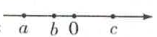
\includegraphics[width=0.3\linewidth]{pic/20200520001.png}. 则\(a,b,c,0\)用`` > '' 连接起来为 \tkt{\(c>0>b>a\)} .
    \item 类别比较法\\
        (1)正数\(>0>\)负数;\\
        (2)两个负数比较大小, \tkt{绝对值大}的反而小\\
        (3)技巧:在实数大小比较中, 若一组数里有正数,0,负数, 最大的数在\tkt{正数}里面选; 最小的数在\tkt{负数}里面选, 即转化为比较正数与正数或负数与负数的大小.
    \item 作差比较法\\
        (1) \(a-b>0 \iff a>b\)\\
        (2) \(a-b=0 \iff a=b\)\\
        (3) \(a-b<0 \iff a<b\)
    \item 平方比较法: \(a>b^2 \iff \)\tkt{\(\sqrt{a}>b(b\ge 0)\)}.(主要用于二次根式的\tkt{估值}及含有\tkt{二次根号}的实数比较大小).
    \item 数字\(-3,0,-\sqrt{3},\pi,3.14,\sqrt{5}\),最小的数是 \tkt{\(-3\)},最大的数是\tkt{\(\pi \)}, 将这些数字用 ``> '' 连接起来 \tkt{\(\pi > 3.14 > \sqrt{5} > 0> -\sqrt{3}>-3\)}
    \end{zsyd}
\end{zsyd}

\chapter{代数式与整式}%
\label{cha:代数式与整式}

\section{知识要点}%
\begin{zsyd}
\item 列代数式与代数式求值
    \begin{zsyd}
    \item 列代数式:把问题中与\tkt{数量}有关的词语, 用含有数,字母和运算符号的式子表示出来, 如:
        \begin{zsyd}
        \item 原量\(a\)增加\(10\%\)为 \tkt{\(a(1+10\%)\)};原量\(a\)减少\(10\%\)为\tkt{\(a(1-10\%)\)} ;比原量\(a\)的\(n\)倍多\(m\)为\tkt{\(na+m\)}; 比原量\(a\)的\(n\)倍少\(m\)为\tkt{\(na-m\)};
        \item 原价\(a\)的八五折为\tkt{\(0.85a\)};原价\(a\)的八折为\tkt{\(0.8a\)};按成本\(a\)提高\(x\%\) 后再打七五折为\tkt{\(0.75a(1+x\%)\)}
        \end{zsyd}
    \item 代数式求值
        \begin{zsyd}
        \item 直接代入法:把已知字母的值, 直接代入代数式, 并按原来的运算顺序计算求值;
        \item \tkt{整体代入}思想:先对比已知定值关系式与所求代数式, 找出两个式子间共同的部分作为切入点, 再对已知关系式与所求代数式进行变形(一般会用到提公因式法. 平方差公式法. 完全平方公式法) ; 然后将已知定值关系式或变形后的式子整体代入计算求值即可.\\
            例:已知 \(x+\frac{1}{x}=3\), 试求 \(x^2+\frac{1}{x^2}\) 和\((x-\frac{1}{x})^2\)的值
\begin{solution}
                \(x+\frac{1}{x}=3 \Rightarrow x^2+\frac{1}{x^2}+2=9 \Rightarrow x^2+\frac{1}{x^2}=7\)\\
                \((x-\frac{1}{x})^2=x^2+\frac{1}{x^2}-2=7-2=5\)
\end{solution}
        \item 常见代数式的隐含条件(代数式的数学意义):
            \begin{zsyd}
            \item \(\frac{1}{a} \Rightarrow \) \tkt{\( a\ne 0\)}, \(\sqrt{a} \Rightarrow \) \tkt{\(a\ge 0\)}.例:求\(\sqrt{a-b}+\sqrt{b-a}\)的值.
            \item 常见的非负数:\tkt{\(\sqrt{a}, |a|, a^2\)}.例:若\(|a|+b^2+\sqrt{c}=0\),求\(a, b,c\)的值.\tkt{\(a=b=c=0\)}
            \end{zsyd}
        \end{zsyd}
    \end{zsyd}
\item 整式基础概念
    \begin{zsyd}
    \item 单项式
        \begin{zsyd}
        \item 定义: 由\tkt{数字与字母的乘积}所组成的代数式.单独一个数字或字母\tkt{也是}单项式.
        \item 系数:单项式中的\tkt{数字因数}.
        \item 单项式的次数:一个单项式中, \tkt{所有字母的指数之和}.单独一个非零常数的次数为\tkt{\(0\)}.例:\(\frac{-3 \times 10^2\pi a^5b}{4}\)的系数与次数.
        \end{zsyd}
    \item 多项式
        \begin{zsyd}
        \item 定义:\tkt{几个单项式的和}.
        \item 多项式项:一个多项式中的\tkt{每个单项式}.不含字母的项叫做\tkt{常数项}.
        \item 次数: 多项式中\tkt{次数最高项的次数}叫做多项式的次数, 如\(a^2+b+c\)的次数是\tkt{\(2\)}.
        \end{zsyd}
    \item 整式:\tkt{单项式与多项式}的统称.
    \item 同类项: \tkt{所含字母相同,且相同字母的指数也相同的项} .所有的常数项\tkt{都是}同类项.
    \end{zsyd}
\item 整式的运算
    \begin{zsyd}
    \item 加减
        \begin{zsyd}
        \item 实质是\tkt{合并同类项}:将同类项的系数 \tkt{相加减} , 字母和字母的 \tkt{指数} 不变;
        \item 遇到括号时, 若括号前面是负号, 则括号内的每一项都要 \tkt{变号} .口诀:``\(-\)'' 变``\(+\)''不变.
        \end{zsyd}
    \item 幂的运算
        \begin{zsyd}
        \item 同底数幂的乘法:底数\tkt{不变},指数\tkt{相加}.\(a^m \cdot a^n = \tkt{a^{m+n}}, \, a^m \cdot a^n \cdot a^p = \tkt{a^{m+n+p}}\);
        \item 同底数幂的乘方: 底数\tkt{不变},指数\tkt{相乘}. \((a^m)^n = \)\tkt{\(a^{mn}\)}
        \item 积的乘方: 积的乘方等于\tkt{乘方的积}. \((ab)^n = \)\tkt{\(a^nb^n\)}
        \item 同底数幂的除法:底数不变,指数相减. \(a^m \div a^n = \)\tkt{\(a^{m-n}\)}
        \item 特殊约定:\(a^0=\)\tkt{\(1(a\ne 0)\)}, \quad \(a^{-p}=\)\tkt{\(\frac{1}{a^p}(a\ne 0)\)}
        \end{zsyd}
    \item 乘法运算
        \begin{zsyd}
        \item 单项式与单项式相乘:把\tkt{系数},\tkt{相同字母}的幂分别相乘,其余字母连同它的\tkt{指数}不变作为积的因式.
        \item 单项式乘法技巧:(1) \tkt{判断符号}; (2)\tkt{计算系数}; (3)\tkt{逐个字母计算次数}
        \item 单项式与多项式相乘:根据\tkt{分配率}用单项式去乘多项式的每一项,再把所得的积相加.
        \item 多项式与多项式相乘:先用一个多项式的每一项乘另一个多项式的每一项,再把所得的积相加.
        \end{zsyd}
    \item 平方差公式与完全平方公式
        \begin{zsyd}
        \item 平方差公式: \tkt{\((a+b)(a-b)=a^2-b^2\)}
        \item 完全平方公式:\tkt{\((a \pm b)^2 = a^2 \pm 2ab + b^2\)}
        \end{zsyd}
    \item 除法运算
        \begin{zsyd}
        \item 单项式除单项式:把\tkt{系数},\tkt{同底数幂}分别相除后,作为商的因式;对于只在被除式里含有的字母,则连同它的指数一起作为商的一个因式.如: \(8m^2n^2 \div 2m^3np = \frac{4n}{mp}\)
        \item 多项式除以单项式,先把多项式的每一项分别除以单项式,再把所得的商相加.如: \( (a^2b+3ab) \div a = ab + 3b \)
        \end{zsyd}
    \end{zsyd}
\item 因式分解
    \begin{zsyd}
    \item 定义:把多项式表示为\tkt{若干个整式的积}的形式.
        \begin{zsyd}
        \item 和差化积:将整式的\tkt{和差}形式化为\tkt{乘积}形式.
        \item 因式分解与\tkt{整式乘法}互为逆运算. \(x(x+y) \leftrightharpoons x^2+xy \),\tkt{从左到右}为整式乘除,\tkt{从右到左}为因式分解.可用整式的乘法运算验证因式分解是否正确.
        \end{zsyd}
    \item 因式分解的方法
        \begin{zsyd}
        \item 提公因式法:
            \begin{zsyd}
            \item 先提\tkt{系数的最大公约数}(如多项式第一项带有负号,应先提取负号);
            \item 再提\tkt{各字母最低的次数};
            \item 提取后观察\tkt{是否可进一步分解}
            \end{zsyd}
        \item 公式法:(1)\tkt{完全平方}公式; (2)\tkt{平方差}公式
        \item 分组分解法
        \item 十字相乘法
            \begin{zsyd}
            \item 只适用于如\tkt{\(ax^2+bx+c\)}形式的二次三项式
            \item 原理:\tkt{\((x+a)(x+b)=x^2+(a+b)x+ab\)}, \tkt{\((ax+b)(cx+d)=acx^2+(ad+bc)x+bd\)},
            \item 两种情况:(1)\tkt{二次项系数为1}; (2)\tkt{二次项系数不为1}
            \item 为一元二次方程,一元二次函数打基础
            \end{zsyd}
        \end{zsyd}
    \end{zsyd}
\end{zsyd}

\chapter{分式}%
\label{cha:分式}

\begin{zsyd}
\item 基本概念
    \begin{zsyd}
    \item 定义:形如\tkt{\(\dfrac{A}{B}\)}的式子,其中\(A,B\)为两个\tkt{整式},\tkt{\(B \ne 0\)},且\tkt{\(B\)中含有字母}.
    \item 分式\(\dfrac{A}{B}\)有意义的条件是: \tkt{\(B\ne 0\)}  ;
    \item 分式\(\dfrac{A}{B}\)值为\(0\)的条件是:  \tkt{\(A=0, B\ne 0\)}  ;
    \item 最简分式: \tkt{分子和分母没有公因式}的分式.
    \item 【易错警示】分式化简时, 要将结果化成\tkt{最简结果}.
    \end{zsyd}
\item 分式的性质
    \begin{zsyd}
    \item 基本性质:分式的分子与分母\tkt{乘(或除以)同一个不等于0的整式},分式的值不变:
    \item 符号变化法则:分式中\tkt{分式本身},\tkt{分子},\tkt{分母}三者有\tkt{两者同时}改变符号,分式值不变.如 \(\frac{2}{3}=\) \tkt{\(\frac{-2}{-3} = -\frac{-2}{3}=-\frac{2}{-3}\)}
    \item 基本性质的应用:通分.\tkt{\(\frac{A}{B}=\frac{A\cdot C}{B\cdot C}\)}.
    \item 基本性质的应用:约分.\tkt{\(\frac{A}{B}=\frac{A \div C}{B \div C}\)},其中\(A, B ,C\)是整式, 且\(c \ne 0\).
    \end{zsyd}
\item 分式的运算法则
    \begin{zsyd}
    \item 通分
        \begin{zsyd}
        \item 通分的概念:根据分式基本性质, 把\tkt{异分母}分式化为与原来的分式\tkt{相等}的\tkt{同分母}分式.
        \item 通分的方法: 关键是寻找\tkt{最简公分母}.\ding{172}各分母能\tkt{因式分解}的先\tkt{因式分解}; \ding{173}取各分母中所有因式的\tkt{最高次幂的积}(数字因式取\tkt{最小公倍数}) 作为公分母.
        \end{zsyd}
    \item 约分
        \begin{zsyd}
        \item 约分的概念:把一个分式分子与分母的\tkt{公因式}约去.
        \item 约分的方法: 关键是寻找分子. 分母的\tkt{公因式}.\ding{172}分子、分母能因式分解的先因式分解; \ding{173}取分子、分母中的\tkt{相同因式的最低次幂的积}(数字因式取\tkt{最大公约数}) 作为公因式.
        \end{zsyd}
    \item 分式的加减运算
        \begin{zsyd}
        \item \tkt{同分母}分式加减:分母不变,分子相加减.\(\frac{a}{c} \pm \frac{b}{c}\)=\tkt{\(\frac{a\pm b}{c}\)}  ;
        \item \tkt{异分母}分式加减:先\tkt{通分},再按同分母分式的加减法则计算.\(\frac{a}{b}\pm \frac{c}{d}\)= \tkt{\(\frac{ad+bc}{bd}\)}
        \end{zsyd}
    \item 分式的乘除运算
        \begin{zsyd}
        \item 乘法运算:分子乘分子,分母乘分母.\(\frac{a}{b}\cdot \frac{c}{d}\)=  \tkt{\(\frac{ac}{bd}\)}  ;
        \item 除法运算:先\tkt{转化为乘法},能\tkt{约分的约分}后再\tkt{按乘法法则}运算,\(\frac{a}{b} \div \frac{c}{d}\) =\tkt{\(\frac{a}{b}\cdot \frac{d}{c}\)} = \tkt{\(\frac{ad}{bc}\)}.
        \end{zsyd}
    \item 分式的混合运算:先\tkt{乘方}, 再乘除, 最后加减; 同级运算从左到右依次进行; 如有括号先计算括号内.
    \end{zsyd}
\end{zsyd}

\part{方程与不等式}%
\label{prt:方程与不等式}

\chapter{一次方程(组)及其应用}%
\label{cha:一次方程(组)及其应用}

\section{知识要点}%

\begin{zsyd}
\item 等式的性质
    \begin{zsyd}
    \item 等式两边加(或减) 同一个数(或式子) , 结果\tkt{仍相等}, 即若\(a=b\),则\(a\pm c\)\tkt{\(=\)}\(b\pm c\)
    \item 等式两边乘同一个数或除以\tkt{同一个不为0}的数, 结果\tkt{仍相等}, 即若\(a = b\),则\(ac\)\tkt{=}\(bc\);若\(a=b(c\ne 0)\),则\(\frac{a}{c}\)\tkt{=}\(\frac{b}{c}\)
    \end{zsyd}
\item 解一元一次方程的步骤
    \begin{zsyd}
    \item \tkt{去分母}.注意不要漏乘不含分母的项, 分子是多项式时注意添括号.
    \item \tkt{去括号}.若括号前是负号, 去括号后括号内各项均要 \tkt{变号}.
    \item \tkt{移项,合并同类项}.移项要\tkt{变号}.
    \item \tkt{系数化为1}.方程两边都除以未知数的系数.
    \end{zsyd}
\item 二元一次方程组的解法
    \begin{zsyd}
    \item 基本思想:二元一次方程\(\xlongrightarrow{\mbox{\text{消元}}}\)一元一次方程.
    \item 代入消元法: 当方程组中一个方程的某一个未知数\tkt{的系数的绝对值是1}或一个方程的\tkt{常数项为零}时,可优先选用代入消元法;
    \item 加减消元法:
        \begin{zsyd}
        \item 当方程组中两个方程的同一未知数的系数的绝对值\tkt{相等}或\tkt{成整数倍}时, 可优先选用加减消元法;
        \item 当方程组中两个方程的两个未知数的对应系数不相等且不成整数倍关系时, 一般选择\tkt{系数绝对值的最小公倍数较小}的未知数消元, 仍选用加减消元法.
        \end{zsyd}
    \end{zsyd}
\item 一次方程组的实际应用:常见基本关系
    \begin{zsyd}
    \item 购买分配类问题:\tkt{\(\begin{cases} \text{数量关系:甲的数量+乙的数量=总数量};\\ \text{费用关系:甲的单价} \times \text{甲的数量}+\text{乙的单价}\times\text{乙的数量}=\text{总费用} \end{cases}\)}
    \item 利润问题 \tkt{\(\begin{cases} \text{售价}=\text{标价} \times \text{折扣;注:八折即标价乘} 80\%,\text{八五折即标价乘}85\% \\ \text{利润}=\text{售价}-\text{进价}; \\ \text{利润率}= \dfrac{\text{利润}}{\text{成本价}} \\ \text{总利润}=(\text{单件售价}-\text{单件进价}) \times \text{销量}\end{cases}\)}
\item 工程问题:\tkt{工作效率} \(\times \) \tkt{工作时间}=工作总量.
    \end{zsyd}
\end{zsyd}

\section{真题}%
\label{sec:真题}

例:(2014江西16题6分)小锦和小丽购买了价格分别相同的中性笔和笔芯.小锦买了\( 20\)支笔和\(2\)盒笔芯,用了\( 56\)元;小丽买了\( 2\)支笔和\(3\)盒笔芯,仅用了\( 28\)元,求每支中性笔和每盒笔芯的价格.
\begin{solution}
    设中性笔和笔芯的价格分别为\(x,y\)元.\\
    \(\begin{cases} 20x+2y=56\\ 2x+3y=28\end{cases}\Rightarrow \begin{cases} x=2\\ y=8\\  \end{cases}\)\\
\end{solution}

\chapter{分式方程及其应用}%
\label{cha:分式方程及其应用}
\begin{note}
    人教:八上第十五章P 149-P 156; 北师: 八下第五章 P 125 - P 130
\end{note}

\begin{zsyd}
\item 分式方程的概念及解法
    \begin{zsyd}
    \item 分式方程的概念:\tkt{分母中含有未知数}的方程.
    \item 解分式方程
        \begin{zsyd}
        \item 基本思想:分式方程\(\xlongrightarrow{\text{化简}}\)整式方程
        \item 一般步骤:
            \begin{zsyd}
            \item 化为\tkt{整式方程:去分母}
            \item 解整式方程
            \item \tkt{检验}:\(\begin{cases} \text{\tkt{最简公分母为0}}:x=a\text{不是分式方程的解}\\ \text{\tkt{最简公分母不为0}}:x=a\text{是分式方程的解} \\  \end{cases}\)
            \end{zsyd}
        \item 技巧:去分母时, 先确定\tkt{最简公分母}; 若分母是多项式, 要进行\tkt{因式分解}; 若分子是多项式,则需将其\tkt{看作一个整体},\tkt{加括号}后再进行下一步运算.
        \item 分式方程的增根:分式方程的增根是\tkt{去分母后的整式方程解得根,但此根却是使分式方程的分母为0的根}.
        \item 分式方程无解:可能是\tkt{解为增根}, 也可能是\tkt{去分母后的整式方程无解}.
        \end{zsyd}
    \end{zsyd}
\item 分式方程的实际应用
    \begin{zsyd}
    \item 解题步骤:实际问题\(\xlongrightarrow[\mbox{\text{设未知数}}]{\mbox{\text{找等量关系}}}\)列分式方程 \(\to\)解分式方程 \(\to\)双检验 \(\to\)作答.
    \item 【易错警示】 解分式方程必须``双检验'' :  \ding{172}检验\tkt{是否是分式方程的解}; \ding{173}检验\tkt{是否符合实际意义}.
    \item 常见问题的关系式
        \begin{zsyd}
        \item 行程问题\tkt{\(\begin{cases} \dfrac{\text{路程}}{\text{速度}}= \text{时间}\\ \dfrac{\text{同一路程}}{\text{慢速}} - \dfrac{\text{同一路程}}{\text{快速}} = \text{时间差} \end{cases}\)}
        \item \(\dfrac{\text{工作总量}}{\text{\tkt{工作效率}}}=\text{工作时间}\)
        \item 购买分配类问题:\tkt{\(\dfrac{\text{总价}}{\text{单价}}=\text{数量}\)}
        \end{zsyd}
    \end{zsyd}
\end{zsyd}

\chapter{一元二次方程及其应用}%
\label{cha:一元二次方程及其应用}
\section{知识要点}%
\label{sec:知识要点}

\begin{zsyd}
\item 一元二次方程的一般形式\tkt{\(ax^2+bx+c=0\)}
\item 一元二次方程的解法
    \begin{zsyd}
    \item 一元二次方程的四种解法:\tkt{直接开平方法},\tkt{因式分解法},\tkt{配方法},\tkt{公式法}
    \item 解法适用情况
        \begin{table}[htbp]
            \centering
            \caption{一元二次方程的解法及适用情况}
            \begin{tabular}{|l|p{36em}|}
                \hline
                \multicolumn{1}{|c|}{\textbf{解法}} & \multicolumn{1}{c|}{\textbf{适用情况}} \bigstrut\\
                \hline
                公式法   & 适用于所有\(b2 -4ac \ge 0\)的一元二次方程, 求根公式为\(x=\) \tkt{\(\frac{-b\pm \sqrt{b^2-4ac}}{2a}\)}  \newline{}【易错警示】 (1)使用求根公式时要先把一元二次方程化为\(ax^2 + bx +c =\tkt{0}(a,b,c为\text{常数, 且} a \ne 0\))的形式; (2)将\(a, b,c\)代入公式时应注意其\tkt{符号} \bigstrut\\
                \hline
                直接开平方法 & 适用于:\newline{}1. \tkt{\(ax^2 + c =0( a \ne 0,ac <0),\)}或 \tkt{\(ax^2 =c(a \ne 0, ac >0)\)};\newline{}2. \tkt{\((x + n)^2 =p(p \ge 0)\)}的方程 \bigstrut\\
                \hline
                配方法   & 配方法适用于所有一元二次方程, 其中当二次项系数\tkt{化为1}后,一次项系数为\tkt{偶数}时用配方法更简单.以\(x^2 + px + q =0\)为例,具体步骤如下:\newline{}(1) 若二次项系数不为1, 先把系数化为1 ;\newline{}(2) 把常数项移到方程的右边, 即\(x^2+px= -q\);\newline{}(3) 在方程两边同时加上一次项系数一半的平方, 即\(x^2 +px + (\frac{p}{2})^2 = -q +(\frac{q}{2})^2\);\newline{}(4) 把方程整理成\((x+ \frac{p}{2})^2 = -q + (\frac{p}{2})^2\)的形式;\newline{}(5) 运用直接开平方法解方程 \bigstrut\\
                \hline
                因式分解法 & 1.缺少常数项, 即方程\(ax^2+bx=0(a \ne 0)\)\newline{} 2.一元二次方程的右边为\(0\),左边易于分解成两个一次因式的乘积;\newline{} 3.方程两边含有相同的因式\newline{}注意: 方程两边不能同时除以含未知数的因式 \bigstrut\\
                \hline
            \end{tabular}%
        \end{table}%
    \item 【易错警示】: 解一元二次方程过程中, 若公因式中含有未知数, 应先移项, 提取公因式, 将方程左边化为因式乘积, 右边为0的形式, 切记\tkt{不能直接约去含有未知数的公因式}, 以免\tkt{丢根}.
    \end{zsyd}
\item 一元二次方程根的判别式:
    \begin{zsyd}
    \item 一元二次方程\(ax^2 +bx+c = 0(a \ne 0)\)的根的判别式为: \tkt{\(b^2-4ac\)}  .
    \item  \(b^2-4ac>0 \)\(\iff\)方程有\tkt{两个不相等的实数根};
    \item  \(b^2-4ac=0 \)\(\iff\)方程有\tkt{两个相等的实数根};
    \item  \(b^2-4ac<0 \)\(\iff\)方程\tkt{无实数根}.
    \item 【易错警示】对于根据方程根的情况确定未知数的值(或范围)时,若二次项系数含有字母,切勿\tkt{忽略二次项系数不为0的条件}.
    \end{zsyd}
\item 一元二次方程根与系数的关系(韦达定理)
    \begin{zsyd}
    \item 若一元二次方程\(ax^2 +bx+c = 0(a \ne 0)\)有两个根分别为\(x_1,x_2\),则\(x_1+x_2\)=\tkt{\(\frac-{b}{a}\)}, \(x_1\cdot x_2\)= \tkt{\(\frac{c}{a}\)}.
    \item 【易错警示】应用根与系数关系的前提是\tkt{方程有实数解},即\tkt{\(b^2 -4ac \ge 0\)}.
    \end{zsyd}
\item —元二次方程实际应用
    \begin{zsyd}
    \item 增长(下降)率问题:设基数为\(a\),平均增长率(下降率)为\(x\),则一次增长(下降)后的值为\tkt{\(a(1\pm x )\)},二次增长(下降)后的值为\tkt{\(a(1\pm x)^2\)};
    \item 面积问题及常见图形:\\
        \ding{172}如图 \ding{172}, 矩形\(ABCD\)长为\(a\),宽为\(b\),设空白部分的宽为\(x\), 则\(S_\text{阴影} = \)\tkt{\((a-2x)(b-2x)\)}.\\
        \ding{173}如图 \ding{173},\ding{174}, 矩形\(ABCD\)长为\(a\),宽为\(b\),设阴影部分的宽为\(x\), 则\(S_\text{空白}=\)\tkt{\((a-x)(b-x)\)}.\\
        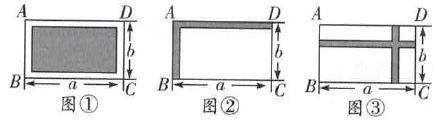
\includegraphics[width=0.5\linewidth]{pic/20200510001.png}
    \end{zsyd}
\end{zsyd}
\chapter{不等式(组)的解法及不等式的应用}%
\label{cha:不等式(组)的解法及不等式的应用}

\begin{note}
    【对接教材】人教:七下第九章P113 - P133 ; 北师: 八下第二章P36-P63.
\end{note}

\begin{zsyd}
\item 不等式的性质
    \begin{zsyd}
    \item 不等式的两边都加(或减)同一个整式,不等号的方向不变,即若\(a>b\),则\(a \pm c =\)\tkt{\(>\)}\(b\pm c\)
    \item 不等式的两边都乘(或除以)同一个正数, 不等号的方向不变.即若\(a>b\),\(c>0\),则\(ac\)\tkt{\(>\)}\(bc\)(或\(\frac{a}{c}\)\tkt{\(>\)}\(\frac{b}{c})\)
    \item 不等式的两边都乘(或除以)同一个负数, 不等号的方向不变.即若\(a>b,c<0\),则 \(ac\) \tkt{\(<\)}\(bc\)(或\(\frac{a}{c}\) \tkt{\(<\)} \(\frac{b}{c}\)) ;
    \item 口诀: 负变正不变
    \end{zsyd}
\item 一元一次不等式的解法及解集表示
    \begin{zsyd}
    \item 解题步骤:\tkt{去分母},去括号,移项,\tkt{合并同类项}, \tkt{系数化为1}.(系数为负则不等号方向改变)
    \item 解集表示:
        \begin{table}[htbp]
            \centering
            \caption{不等式解集的数轴表示}
            \begin{tabular}{|l|p{12em}|}
                \hline
                \multicolumn{1}{|c|}{\textbf{解集}} & \textbf{数轴表示} \bigstrut\\
                \hline
                \(x<a\)   & 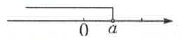
\includegraphics[width=0.5\linewidth]{pic/20200510002.png} \bigstrut\\
                \hline
                \(x\le a\)  & 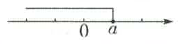
\includegraphics[width=0.5\linewidth]{pic/20200510004.png} \bigstrut\\
                \hline
                \(x>a\)   &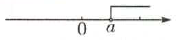
\includegraphics[width=0.5\linewidth]{pic/20200510003.png} \bigstrut\\
                \hline
                \(x\ge a\)  & 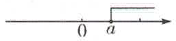
\includegraphics[width=0.5\linewidth]{pic/20200510005.png} \bigstrut\\
                \hline
            \end{tabular}%
            \label{tab:addlabel}%
        \end{table}%
    \item 注意:实心圆点与空心圆点的区别:\tkt{空心}圆点\(\iff “>”\text{或}“<”\);\tkt{实心}圆点\(\iff “\ge ”\text{或}“\le ”\)
    \end{zsyd}
\item 不等式组的解法及解集表示
    \begin{zsyd}
    \item 解题步骤:一元一次不等式组 \(\to \)解每个一元一次不等式 \(\to \) \tkt{确定各不等式解集的公共部分}\(\to \) 写出一元一次不等式组的解集
    \item 解集表示:
        \begin{table}[H]
            \centering
            \caption{一元一次不等式组解集及数轴上的表示}
            \begin{tabular}{|l|p{10em}|p{10em}|p{10em}|}
                \hline
                \multicolumn{1}{|c|}{\textbf{解集(\(a>b\))}} & \textbf{数轴表示} & \multicolumn{1}{c|}{\textbf{解集}} & \multicolumn{1}{c|}{\textbf{口诀}} \bigstrut\\
                \hline
                \(\begin{cases} x\ge a\\ x>b \end{cases}\) & 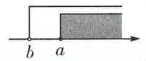
\includegraphics[width=0.5\linewidth]{pic/20200510006.png}     &   \tkt{\(x\ge a\)}   & 同大取大 \bigstrut\\
                \hline
                \(\begin{cases} x\le a\\ x < b \end{cases}\)  & 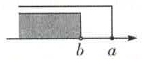
\includegraphics[width=0.5\linewidth]{pic/20200510007.png}     &   \tkt{\(x<b\)}   & 同小取小 \bigstrut\\
                \hline
                \(\begin{cases} x < a\\ x\ge b \end{cases}\)   & 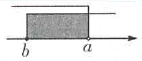
\includegraphics[width=0.5\linewidth]{pic/20200510008.png}     &  \tkt{\(b\le x<a\)}    & 大小小大中间找 \bigstrut\\
                \hline
                \(\begin{cases} x > a\\ x \le b \end{cases}\)  & 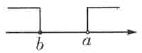
\includegraphics[width=0.5\linewidth]{pic/20200510009.png}     &  \tkt{无解}    & 大大小小无处找 \bigstrut\\
                \hline
            \end{tabular}%
            \end{table}%
    \end{zsyd}
\item 一元一次不等式的实际应用:\\
    \begin{table}[H]
        \centering
        \caption{常见关键词与不等号的对应关系}
        \begin{tabular}{|c|p{12em}|}
            \hline
            \textbf{常用关键词} & \textbf{符号} \bigstrut\\
            \hline
            大于, 多于, 超过, 高于 &  > \bigstrut\\
            \hline
            小于, 少于, 不足, 低于 & < \bigstrut\\
            \hline
            至少, 不低于, 不小于,不少于 & >= \bigstrut\\
            \hline
            至多,不超过, 不高于, 不大于 & <= \bigstrut\\
            \hline
        \end{tabular}%
        \label{tab:addlabel}%
    \end{table}%
\end{zsyd}

\part{函数}%
\label{prt:函数}

\chapter{平面直角坐标系及函数}%
\label{cha:平面直角坐标系及函数}
\section{知识要点}%
\begin{zsyd}
\item 点的坐标特征
    \begin{zsyd}
    \item 各象限内的点的坐标轴符号\\
        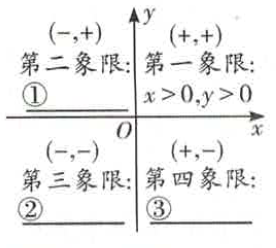
\includegraphics[width=0.2\linewidth]{pic/20200510011.png}
        \begin{zsyd}
        \item 第一象限: \tkt{\((+,+)\)}
        \item 第二象限: \tkt{\((-,+)\)}
        \item 第三象限: \tkt{\((-,-)\)}
        \item 第四象限: \tkt{\((+,-)\)}
        \end{zsyd}
    \item 坐标轴上的点\\
        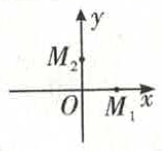
\includegraphics[width=0.2\linewidth]{pic/20200510012.png}
        \begin{zsyd}
        \item 点在x轴上:\tkt{纵坐标为0},即\tkt{\((x,0)\)}
        \item 点在y轴上:\tkt{横坐标为0},即\tkt{\((0,y)\)}
        \item 原点坐标:(0,0)
        \end{zsyd}
    \item 各象限角平分线上的点\\
        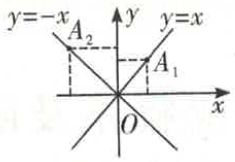
\includegraphics[width=0.2\linewidth]{pic/20200510013.png}
        \begin{zsyd}
        \item 第一,三象限角平分线上的点:\tkt{横纵坐标相等},即\tkt{\((x,x)\)}
        \item 第二,四象限角平分线上的点:\tkt{横纵坐标互为相反数},\tkt{\((x,-x)\)}
        \end{zsyd}
    \item 与坐标轴平行的直线上的点\\
        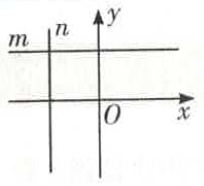
\includegraphics[width=0.2\linewidth]{pic/20200510014.png}
        \begin{zsyd}
        \item 平行于x轴上的直线\(m\)上的点的\tkt{纵}坐标相同,即\tkt{\(x,m\)}
        \item 平行于y轴上的直线\(n\)上的点的\tkt{横}坐标相同,即\tkt{\(n,y\)}
        \end{zsyd}
    \item 平面直角坐标系上任意两点\(A(x_1,y_1),B(x_2,y_2)\)的中点坐标为\(\frac{x_1+x_2}{2},\frac{y_1+y_2}{2}\)
    \item 某点\((x_1,y_1)\)绕定点\((a,b)\)旋转\(180^\circ\)得到的对应点(\(x_2,y_2)\)的坐标可借助中点坐标求解得:\tkt{\(x_2=2a-x_1,y_2=2b-y_1\)}.
    \end{zsyd}
\item 坐标系中的距离公式
    \begin{zsyd}
    \item 点到坐标轴的距离\\
        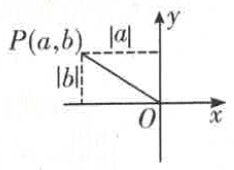
\includegraphics[width=0.2\linewidth]{pic/20200510015.png}
        \begin{zsyd}
        \item 点\(P(a, b)\)到\(x\)轴的距离为\tkt{\(|b|\)}
        \item 点\(P(a, b)\)到\(y\)轴的距离为\tkt{\(|a|\)}
        \item 点\(P(a, b)\)到原点的距离为\tkt{\(\sqrt{a^2+b^2}\)}
        \end{zsyd}
    \item 平行于坐标轴的直线上两点间的距离\\
        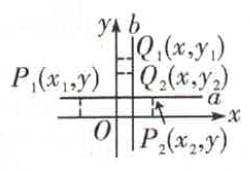
\includegraphics[width=0.2\linewidth]{pic/20200510016.png}
        \begin{zsyd}
        \item 平行于x轴的直线m上的两点\(P_1(x_1,y),P_2(x_2,y)\) \(\iff\)纵坐标恒相等, \(P_1P_2 =\) \(|x_1-x_2|\)
        \item 平行于x轴的直线n上的两点\(Q_1(x,y_1),Q_2(x,y_2)\) \(\iff\)横坐标恒相等, \(Q_1Q_2 =\) \(|y_1-y_2|\)
        \end{zsyd}
    \item 坐标系中任意两点\(P_1(x_1,y_1),P_2(x_2,y_2),\)间的距离\(|P_1P_2|=\)\(\sqrt{(x_1-x_2)^2+(y_1-y_2)^2}\)\\
        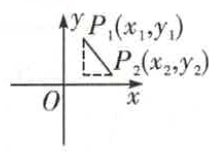
\includegraphics[width=0.2\linewidth]{pic/20200510017.png}
    \end{zsyd}
\item 点的平移
    \begin{zsyd}
    \item 将点\(P(x,y)\)向左平移\(a(a >0)\)个单位长度后对应点为\(P'\)\tkt{\((x-a,y)\)}  ;
    \item 将点\(P(x,y)\)向右平移 \(a(a >0)\)个单位长度后对应点为\(P'\) \tkt{\((x+a,y)\)}  ;
    \item 将点\(P(x,y)\)向上平移\(b(b>0)\)个单位长度后对应点为\(P'\)  \tkt{\((x,y+b)\)} ;
    \item 将点\(P(x,y)\)向下平移\(b(b>0)\)个单位长度后对应点为\(P'\)  \tkt{\((x,y-b)\)} ;
    \item 将点\(P(x,y)\)先向左平移\(a(a >0)\)个单位长度, 再向上平移\(b(b >0)\)个单位长度后对应点为\(P'\)\tkt{\((x-a,y+b)\)};
    \item 将点\(P(x,y)\)先向右平移 \(a(a >0)\)个单位长度, 再向下平移\(b(b>0)\)个单位长度后对应点为\(P'\)\tkt{\((x+a,y-b)\)}.
    \item 口诀:``左减右加, 上加下减''(注意与函数图像平移的口诀相区分)
    \end{zsyd}
\item 点的对称
    \begin{zsyd}
    \item \(P(a, b)\xlongrightarrow{\mbox{\text{关于\(x\)轴对称}}} P'\)\tkt{\(( a,-b )\)}
    \item \(P(a, b)\xlongrightarrow{\mbox{\text{关于\(y\)轴对称}}} P'\)\tkt{\(( -a,b )\)}
    \item \(P(a, b)\xlongrightarrow{\mbox{\text{关于原点对称}}} P'\)\tkt{\(( -a,-b )\)}
    \item \(P(a, b)\xlongrightarrow{\mbox{\text{关于直线\(y=x\)对称}}} P'\)\tkt{\(( b,a )\)}
    \item \(P(a, b)\xlongrightarrow{\mbox{\text{关于直线\(y=-\)x对称}}} P'\)\tkt{\(( -b,-a )\)}
    \item \(P(a, b)\xlongrightarrow{\mbox{\text{关于直线\(x=m\)对称}}} P'\)\tkt{\(( 2m-a,b )\)}
    \item \(P(a, b)\xlongrightarrow{\mbox{\text{关于直线\(y=n\)对称}}} P'\)\tkt{\(( a,2m-b )\)}
    \end{zsyd}
\item 函数的表示及其图像
    \begin{zsyd}
    \item 函数的表示方法:(1)\tkt{解析式}法; (2)列表法; (3)\tkt{图像}法
    \item 函数图像画法:描点法.(1)列表; (2)描点; (3)连线
    \end{zsyd}
\item 函数自变量取值范围
    \begin{zsyd}
    \item 含分式,形如\(y=\frac{a}{x}\):使\tkt{分母不为零}的实数
    \item 含二次根式,形如\(y=\sqrt{x}\):使\tkt{被开方数大于等于0}的实数
    \item 含分式与二次根式,形如\(y=\frac{a}{\sqrt{x}}\)或\(y=\frac{\sqrt{x+a}}{x}\):使分母\tkt{不为零},且被开方数\tkt{大于等于零}的实数
    \end{zsyd}
\end{zsyd}

\chapter{一次函数及其应用}%
\label{cha:一次函数及其应用}
\section{知识要点}%
\label{sec:知识要点}

\begin{zsyd}
\item 定义:形如\tkt{\(y = kx+b\)}(\(k\),\(b\)为常数,且\tkt{\(k \ne 0\)})的函数.(特别的,当\tkt{\(b=0\)}时, \tkt{\(y=kx\)}为正比例函数,图像过原点.
\item 图形与性质\\
    \begin{table}[H]
        \centering
        \caption{一次函数图像分类}
        \begin{tabular}{|p{6em}|p{5em}|p{5em}|p{5em}|p{5em}|p{5em}|p{5em}|}
            \hline
            k决定图像的倾斜方向和增减性 & \multicolumn{3}{c|}{\(k>0 \iff \begin{cases} \text{图像从左向右上升趋势} \\ y\text{随}x\text{的增大而\tkt{增大}} \\  \end{cases}\)} & \multicolumn{3}{c|}{\(k<0 \iff \begin{cases} \text{图像从左向右下降趋势} \\ y\text{随}x\text{的增大而\tkt{减小}} \\  \end{cases}\)} \bigstrut\\
            \hline
            b决定图像与y轴的交点 & b>0\(\iff\)交点在y轴正半轴 & b=0 \(\iff\)交点在原点 & b<0 \(\iff\)交点在y轴负半轴  & b>0 \(\iff\)交点在y轴正半轴  & b=0 \(\iff\)交点在原点 & b<0 \(\iff\)交点在y轴负半轴\bigstrut\\
            \hline
            图像    &      &      &      &      &      &  \bigstrut\\
            \hline
            经过的象限 & \tkt{一、二、三} & \tkt{一、三} & \tkt{一、三、四} & \tkt{一、二、四} & \tkt{二、四} & \tkt{二、三、四} \bigstrut\\
            \hline
        \end{tabular}%
    \end{table}%
\item 一次函数解析式的确定:\textbf{待定系数法}
    \begin{zsyd}
    \item 一设:设一次函数的解析式为\(y = kx+b,(k\ne 0)\)(题干中未给解析式时需设)
    \item 二列:把已知条件(图象上的点坐标)代入所设解析式中得到含待定系数的方程组
    \item 三解:解方程组求待定系数\(k,b\)的值
    \item 四还原:将所求待定系数的值代入所设的函数解析式中,从而写出函数解析式
    \item 【技巧】若为正比例函数(图象过原点),设解析式为\(y = kx\)(\(k \ne O\)),代入除原点外任意一点坐标即可求解.
    \end{zsyd}
\item 图象的平移:口诀:\textbf{左加右减,上加下减}(注意与点的平移区分)
    \begin{zsyd}
    \item 左右平移\\
        \(y=k(x+m)+b \xlongleftarrow[\mbox{只给x加m}]{\mbox{向左平移m个单位}} y=kx+b \xlongrightarrow[\mbox{只给x减m}]{\mbox{向右平移m个单位}}y=k(x-m)+b \)
    \item 上下平移\\
        \(y=kx+b+n \xlongleftarrow[\mbox{表达式整体加n}]{\mbox{向上平移n个单位}} y=kx+b \xlongrightarrow[\mbox{表达式整体减n}]{\mbox{向下平移n个单位}}y=kx+b-n \)
    \end{zsyd}
\item 与方程(组),不等式的关系
    \begin{zsyd}
    \item 与方程(组)的关系
        \begin{zsyd}
        \item 一次函数\(y = kx + b\)图象与\(x\)轴交点的\tkt{横}坐标是方程\(kx + b=0\)的解
        \item 一次函数\(y = kx + b\)与\(y=k_1x+b_1\)图象\( \tkt{\text{交点横纵坐标值}} \)是方程组\(\begin{cases} y = kx + b\\ y=k_1x+b_1 \end{cases}\) 的解
        \end{zsyd}
    \item 与不等式的关系
        \begin{zsyd}
        \item 不等式\(kx + b>0\)的解集是一次函数\(y = kx + b\)位于\tkt{x轴上方}的图象所对应的自变量的取值范围
        \item 不等式\(kx + b<0\)的解集是一次函数\(y = kx + b\)位于\tkt{x轴下方}的图象所对应的自变量的取值范围
        \item 不等式\(kx + b>k_1x+ b\)的解集是一次函数\(y = kx+b\)的图象位于\(y = k_1x + b_1\)的图象\tkt{上方}部分对应的\(x\)的取值范围
        \item 不等式\(kx+b<k_1x + b\)的解集是一次函数\(y = kx + b\)的图象位于\(y = k_1x + b_1\)的图象\tkt{下方}部分对应的\(x\)的d取值范围
        \end{zsyd}
    \end{zsyd}
\end{zsyd}

\chapter{反比例函数}%
\label{cha:反比例函数}
\begin{note}
    【对接教材】 人教: 九下第二十六章Pl -P22;北师: 九上第六章P149-P162.
\end{note}
\begin{zsyd}
\item 图像与性质
    % Table generated by Excel2LaTeX from sheet '反比例函数'
    \begin{table}[H]
        \centering
        \caption{反函数的图像与性质}
        \begin{tabular}{|p{5em}|c|c|}
            \hline
            \textbf{表达式} & \multicolumn{2}{c|}{\(y=k/x(k\text{为常数,且}k \ne 0)\)} \bigstrut\\
            \hline
            \textbf{图} & \multicolumn{1}{l|}{} & \multicolumn{1}{l|}{} \bigstrut\\

            \hline
            \textbf{k的符号} & \multicolumn{1}{l|}{\(k>0\)} & \multicolumn{1}{l|}{\(k<0\)} \bigstrut\\
            \hline
            \textbf{所在象限} & \multicolumn{1}{l|}{第一、三象限\((xy>0)\)} & \multicolumn{1}{l|}{第二、四象限\((xy<0)\)} \bigstrut\\
            \hline
            \textbf{增减性} & \multicolumn{1}{l|}{每个象限内,y随x的增大而增大} & \multicolumn{1}{l|}{每个象限内,\(y\)随\(x\)的增大而减小} \bigstrut\\
            \hline
            \textbf{图像上的点坐标特征} & \multicolumn{2}{c|}{横,纵坐标乘积为\tkt{\(k\)}} \bigstrut\\
            \hline
            \textbf{\(x,y\)的取值范围} & \multicolumn{2}{c|}{\(x \ne 0, y \ne 0\)} \bigstrut\\
            \hline
            \textbf{对称性} & \multicolumn{2}{c|}{关于直线\tkt{\(y=x, y=-x\)}成轴对称,关于\tkt{原点}成中心对称} \bigstrut\\
            \hline
        \end{tabular}%
    \end{table}%
\item 系数\(k\)的几何意义
    % Table generated by Excel2LaTeX from sheet '反比例函数'
    \begin{table}[H]
        \centering
        \caption{反比例函数k的几何意义}
        \begin{tabular}{|c|c|c|c|}
            \hline
            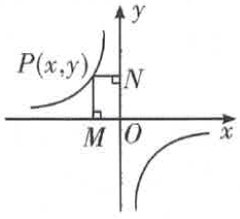
\includegraphics[width=0.15\linewidth]{pic/20200510018.png}     & 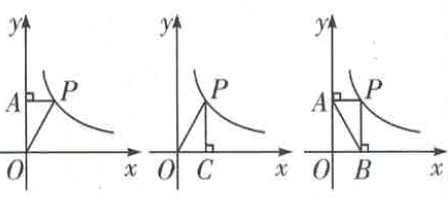
\includegraphics[width=0.4\linewidth]{pic/20200510019.png} & 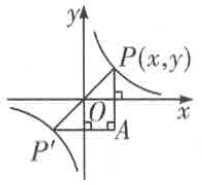
\includegraphics[width=0.15\linewidth]{pic/20200510020.png} & 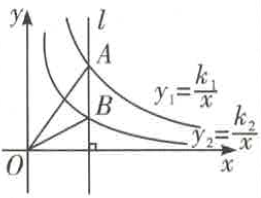
\includegraphics[width=0.15\linewidth]{pic/20200510021.png}
            \bigstrut\\
            \hline
            \(S_{OMNP}=\)\tkt{\(|x_p|\cdot |y_p|=|k|\)} & \(S_{\triangle AOP}=S_{\triangle OCP}=S_{\triangle APB}\)=\tkt{\(\frac{|k|}{2}\)}     & \(S_{\triangle APB}\)=\tkt{\(2|k|\)}     &\(S_{\triangle AOB}=\)\tkt{\(\frac{1}{2}|k_1-k_2|\)}  \bigstrut\\
            \hline
        \end{tabular}%
    \end{table}%
    \textbf{以上图形面积仅与\tkt{\(k\)}有关,与\(P\)点坐标无关}
\item 解析式的确定
    \begin{zsyd}
    \item 待定系数法\\
        \ding{172}设解析式为\(y=\frac{k}{x}(k\ne 0)\)\\
        \ding{173}找出反比例函数图象上的一点\(P(a,b)\)\\
        \ding{174}将\(P(a,b)\)代入解析式得\(k = ab\)\\
        \ding{175}确定反比例函数解析式\(y=\frac{ab}{x}\)
    \item 利用\(k\)的几何意义求解: 当已知面积时可考虑用\(k\)的几何意义.由面积得\(|k|\),再结合图象所在象限判断\(k\)的正负, 从而得出\(k\)值, 代入解析式即可
    \end{zsyd}
\end{zsyd}

\chapter{二次函数图像与性质}%
\label{cha:二次函数图像与性质}
\begin{note}
    【对接教材】 人教: 九上第二十二章P27-P57;北师: 九下第二章P29-P45、P51 -P63.
\end{note}

\begin{zsyd}
\item 定义:形如\tkt{\(y = ax^2 +bx+c(a,b,c\text{是常数,且}a\ne 0)\)},则称\(y\)是\( x \)的二次函数
\item 二次函数图像的基本性质
    \begin{table}[H]
        \centering
        \caption{二次函数图像基本性质}
        \begin{tabular}{|p{6em}|p{15em}|p{15em}|}
            \hline
            \multicolumn{3}{|p{36em}|}{二次函数\(y = ax^2 +bx+c,(a,b, c\text{是常数,且}a \ne 0)\)(各项系数包括它前面的加减号)} \bigstrut\\
            \hline
            图象(草图) &  \(a >0\) & \(a <0\) \bigstrut\\
            \hline
            对称轴   & \multicolumn{2}{p{30em}|}{直线\(x = \)\tkt{\(\frac{-b}{2a}\)}或\(x =\)\tkt{\(\frac{x_1+x_2}{2}\)}(其中\(x_1, x_2\)为\tkt{纵坐标相等}的两个点对应的横坐标)} \bigstrut\\
            \hline
            顶点坐标  & \multicolumn{2}{p{30em}|}{1. 顶点坐标(\tkt{\(\frac{-b}{2a}\)},\tkt{\(\frac{4ac-b^2}{4a}\)})\newline{}2. 运用配方法将一般式转化为顶点式求解} \bigstrut\\
            \hline
            增减性(可画出草图判断)  & 在对称轴左侧,\tkt{y随x的增大而减小}; \newline{} 在对称轴右侧, \tkt{y随x的增大而增大} & 在对称轴左侧,\tkt{y随x的增大而增大};\newline{} 在对称轴右侧,\tkt{y随x的增大而减小} \bigstrut\\
            \hline
            最值    & 当\(x=\frac{-b}{2a}\)时,\(y\)的最小值为\(\frac{4ac-b^2}{4a}\)  & 当\(x=\frac{-b}{2a}\)时,\(y\)的最大值为\(\frac{4ac-b^2}{4a}\) \bigstrut\\
            \hline
        \end{tabular}%
        \label{tab:addlabel}%
    \end{table}%
\item 根据二次函数图像判断\(a,b,c\)的关系式与\(0\)的关系
    \begin{zsyd}
    \item \(a\)的正负决定开口方向
        \begin{zsyd}
        \item 开口向上\( a \tkt{>}  0\)
        \item 开口向下\( a \tkt{<}  0\)
        \end{zsyd}
    \item \(a,b\)决定对称轴位置
        \begin{zsyd}
        \item 对称轴为\(y\)轴\tkt{\( b=0\)}
        \item 对称轴在\(y\)轴左侧\tkt{\(ab<0\)}
        \item 对称轴在\(y\)轴右侧\tkt{\(ab>0\)}
        \end{zsyd}
    \item \(c\)决定与\(y\)轴交点位置
        \begin{zsyd}
        \item 抛物线过原点\( c=0\)
        \item 抛物线与\(y\)轴交于正半轴\( c \tkt{>} 0\)
        \item 抛物线与\(y\)轴交于负半轴\( c \tkt{<} 0\)
        \end{zsyd}
    \item \(b2 -4ac \)决定与\(x\)轴交点个数
        \begin{zsyd}
        \item 与\(x\)轴有唯一交点(顶点)\(b^2-4ac = 0 \)
        \item 与\(x\)轴有两个交点\( b^2-4ac > 0 \)
        \item 与\(x\)轴没有交点\( b^2-4ac < 0 \)
        \end{zsyd}
    \end{zsyd}
\item 特殊代数式正、负的判断方法
    \begin{zsyd}
    \item \(2a+b\):\tkt{\(\dfrac{-b}{2a}\)}与\(1\)比较大小(结合开口方向)
    \item \( 2a- b\):\tkt{\(\frac{-b}{2a}\)}与\(-1\)比较大小(结合开口方向)
    \item \(a+b+c\):令\tkt{\(x=1\)},看纵坐标正负
    \item \(a - b + c \):令\tkt{\(x=-1\)},看纵坐标正负
    \item \(4a+2b+c\)令\tkt{\(x=2\)},看纵坐标正负
    \item \(4a-2b+c\)令\tkt{\(x=-2\)},看纵坐标正负
    \end{zsyd}
\item 二次函数与一元二次方程,不等式的关系
    \begin{zsyd}
    \item 与一元二次方程的关系
        \begin{zsyd}
        \item 抛物线\(y=ax^2+bx+c \)与\(x\)轴交点的横坐标值\(\iff\)一元二次方程\(ax^2+bx+c=0\)的解
        \item \( b^2-4ac > 0 \),抛物线与\(x\)轴有\tkt{两个交点},方程有\tkt{两个不相等}的实数根
        \item \( b^2-4ac = 0 \),抛物线与\(x\)轴有\tkt{一个交点},方程有\tkt{两个相等}的实数根
        \item \(b2 -4ac <0\)抛物线与\(x\)轴\tkt{没有交点},方程\tkt{无实数根}
        \end{zsyd}
    \item 与不等式的关系
        \begin{zsyd}
        \item \(ax^2+bx+c>0\)的解集是抛物线\(y = ax^2+bx+c\)位于\tkt{\(x\)轴上方}的图像对应的\(x\)的取值范围
        \item \(ax^2+bx+c<0\)的解集是抛物线\(y = ax^2+bx+c\)位于\tkt{\(x\)轴下方}的图形对应的\(x\)的取值范围
        \end{zsyd}
    \end{zsyd}
\end{zsyd}

\chapter{二次函数图象的平移,旋转,翻折与解析式的确定}%

\begin{note}
    【对接教材】 人教: 九上第二十二章P32-P42; 北师: 九下第二章P35-P45.
\end{note}

\begin{zsyd}
\item 解析式的确定
    \begin{zsyd}
    \item \tkt{一般式}:\tkt{\(y=ax^2+bx+c (a,b, c \text{为常数,且} a \ne 0)\)}
    \item \tkt{顶点式}:\tkt{\(y = a(x-h)2+k(a,h,k\text{为常数, 且}a \ne 0)\)}其中\((h, k)\)是抛物线的顶点坐标
    \item \tkt{交点式}:\tkt{\(y=a(x-x_1)(x-x_2)(a \ne 0)\)},\(a\)为常数,\(x_1,x_2\)为抛物线与\(x\)轴的\tkt{两个交点的横坐标}
    \end{zsyd}
\item 确定二次函数解析式的方法
    \begin{zsyd}
    \item 解析式未知
        \begin{zsyd}
        \item 顶点在原点, 可设为\tkt{\(y=ax^2\)}
        \item 对称轴是\(y\)轴(或顶点在\(y\)轴上), 可设为\tkt{\(y=ax^2+c\)}
        \item 顶点在\(x\)轴上, 可设为\tkt{\(y=a(x-h)^2\)}
        \item 抛物线过原点, 可设为\tkt{\(y = ax^2+bx\)}
        \item 已知顶点坐标为\((h,k)\)时,可设为顶点式\tkt{\(y = a(x-h)^2 +k\)}
        \item 已知抛物线与\(x\)轴的两交点坐标为\((x_1,0),(x_2,0)\),时可设为交点式\tkt{\(y =a(x-x_1)(x -x_2)\)}
        \end{zsyd}
    \item 解析式已知:解析式中有几个字母未知, 只需找出二次函数图象上相同个数的点的坐标代入求解即可
    \end{zsyd}
\item 二次函数图象的平移:顶点式\(y = a(x-h)^2 +k, m>0\)
    \begin{zsyd}
    \item 口诀:\(左加右减, 上加下减\)
    \item 向左平移\(m\)个单位 \tkt{\(y = a(x -h + m)^2 + k\)}
    \item 向右平移\(m\)个单位 \tkt{\(y = a(x -h - m)^2 + k\)}
    \item 向上平移\(m\)个单位 \tkt{\(y = a(x -h )^2 + k+ m\)}
    \item 向下平移\(m\)个单位 \tkt{\(y = a(x -h )^2 + k- m\)}
    \item 【技巧】 二次函数图象的平移, 其实质是图象上点的整体平移(一般研究\tkt{顶点坐标}, 平移过程\tkt{\(a\)}保持不变), 因此可先求出其\tkt{顶点坐标}, 根据顶点的平移求得函数解析式.
    \end{zsyd}
\item 二次函数图象的旋转,翻折:顶点式\(y = a(x-h)^2 +k, a \ne 0\)
    \begin{zsyd}
    \item 绕顶点旋转\(180 ^\circ\):\tkt{\(y = -a(x -h)^2 +k\)} ,规律:\tkt{\(a\)变号,\(h,k\)均不变}
    \item 绕原点旋转\(180^\circ\):\tkt{\(y = -a(x+h)^2 -k\)} ,规律:\tkt{\(a,h,k\)均变号}
    \item 沿\(x\)轴翻折:\tkt{\(y = -a(x -h)^2 -k\)},规律:\tkt{\(a,k\)变号,\(h\)不变}
    \item 沿\(y\)轴翻折:\tkt{\(y = a(x+h)^2 +k\)},规律:\tkt{\(a,k\)不变,\(h\)变号}
    \end{zsyd}
\item 判断二次函数图象恒过定点的方法:
    \begin{zsyd}
    \item 二次函数\(y=ax^2+bx+c\)(\(a\),\(b\),\(c \)为常数,\(a \ne 0\)),令\(x =0,y=c\)恒成立,故无论\(a,b\)取何值,该函数图象恒过定点\tkt{(\(0\),\(c\))}
    \item 一般地,解析式需化成\tkt{\(y = a(x+b)^2+c\)}的形式,令\tkt{\(x=-b\)},则\tkt{\(y = c\)},无论\(a\)取何值(不为\(0\)),该函数图象恒过定点\tkt{(\(-b,c\))}
    \item 二次函数解析式中的各项有\tkt{公因式},可化成,\tkt{\(y=a(x-m)(x-n)\)}的形式,令\tkt{\(y=0\)},则\tkt{\(x_1=m,x_2=n\)},故无论\(a\)取何值(不为\(0\)),该函数图象恒过定点\tkt{\((m,0)\)}和\tkt{\((n,0)\)}
    \end{zsyd}
\end{zsyd}


\part{三角形}%
\label{prt:三角形}

\chapter{线段,角,相交线与平行线}%
\label{cha:线段,角,相交线与平行线}
\begin{note}
    【对接教材】 人教: 七上第四章P125 -P141, 七下第五章Pl -P27,八上第十二章P48 -P52.P60 - P62; 北师: 七上第四章P106-P121,七下第二章P38-P54,八上第七章P161 -P177,八下第一章P15 -P16.P22 一 P35.
\end{note}
\begin{zsyd}
\item 直线与线段
    \begin{zsyd}
    \item 两个基本事实
        \begin{zsyd}
        \item 直线的基本事实:\tkt{经过两点有且只有一条直线}(简记: \tkt{两点确定一条直线})
        \item 线段的基本事实:\tkt{两点之间的所有连线中线段最短}(简记:\tkt{两点之间线段最短})
        \end{zsyd}
    \item 线段的中点: 如图 \ding{172}, 点\(B\)把线段\(AC\)分成相等的两条线段\(AB\)与\(BC\),点B叫做线段AC的\tkt{中点},即有\tkt{\(AB=BC=\frac{1}{2}AC\)}\\
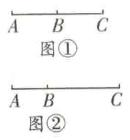
\includegraphics[width=0.15\linewidth]{pic/20200519001.png}
    \item 线段的和与差: 如图 \ding{173},在线段\(AC\)上取一点\(B\),则有\(AB+\)\tkt{\(BC\)}\(=AC\); \(AB=\)\tkt{\(AC\)}\(-BC\); \(AC-AB=\)\tkt{\(BC\)}
    \end{zsyd}
\item 角及角平分线
    \begin{zsyd}
    \item 余角
        \begin{zsyd}
        \item 定义: 如果\tkt{两个角的和}等于\(90^\circ\).那么这两个角互为余角.
        \item 性质: 同角(等角)的余角\tkt{相等}
        \end{zsyd}
    \item 补角
        \begin{zsyd}
        \item 定义: 如果两个角的和等于\tkt{\(180 ^\circ\)},那么这两个角互为补角.
        \item 性质: 同角(等角)的补角\tkt{相等}
        \end{zsyd}
    \item 角平分线
        \begin{zsyd}
        \item 定义: 从一个角的\tkt{顶点}引出一条\tkt{射线},把这个角分成\tkt{两个完全相同的角},这条射线叫做这个角的角平分线.
        \item 性质:\tkt{角平分线上的点到角两边的距离相等}.
        \item 逆定理:角的内部到角两边\tkt{距离相等}的点在角的平分线上
        \end{zsyd}
    \end{zsyd}
\item 相交线
    \begin{zsyd}
    \item 角
        \begin{zsyd}
        \item 对顶角性质:对顶角 \tkt{相等}
        \item 邻补角性质:邻补角之和等于\tkt{\(180^\circ\)}
        \end{zsyd}
    \item 垂线性质
        \begin{zsyd}
        \item 在同一平面内, 过一点\tkt{有且只有一条}直线与已知直线垂
        \item 连接直线外一点与直线上各点的所有线段中,\tkt{垂线段}最短
        \item 点到直线的距离:\tkt{直线外一点到这条直线的垂线段的长度}
        \end{zsyd}
    \item 垂直平分线
        \begin{zsyd}
        \item 性质:\tkt{线段垂直平分线上的点到这条线段两个端点的距离相等}
        \item 判定:\tkt{到一条线段两个端点距离相等}的点,在这条线段的垂直平分线上
        \end{zsyd}
    \item 三线八角\\
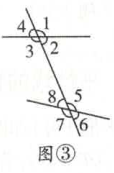
\includegraphics[width=0.15\linewidth]{pic/20200519002.png}
        \begin{zsyd}
        \item 同位角:\(\angle 1\)与\tkt{\(\angle 5\)}, \(\angle 2\)与\tkt{\(\angle 6\)},\(\angle 3\)与\tkt{\(\angle 7\)},\(\angle 4\)与\tkt{\(\angle 8\)}
        \item 内错角:\(\angle 2\)与\tkt{\(\angle 8\)},\(\angle 3\)与\tkt{\(\angle 5\)}
        \item 同旁内角:\(\angle 3\)与\tkt{\(\angle 8\)},\(\angle 2\)与\tkt{\(\angle 5\)}
        \end{zsyd}
    \end{zsyd}
\item 平行线
    \begin{zsyd}
    \item 两个基本事实
        \begin{zsyd}
        \item 公理:经过直线外一点,\tkt{有且只有一条}直线与这条直线平行
        \item 推论:如果两条直线都与第三条直线平行,那么这两条直线也互相平行, 即如果 \(b // a,c // a\),那么\tkt{\(b // c\)}
        \item 注:在同一平面内, \tkt{垂直同一直线}的两条直线平行
        \end{zsyd}
    \item 平行线的性质与判定\\
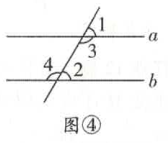
\includegraphics[width=0.15\linewidth]{pic/20200519003.png}
        \begin{zsyd}
        \item \tkt{同位角相等}\(\iff\)两直线平行:
        \item \tkt{内错角相等}\(\iff\)判定 两直线平行:
        \item \tkt{同旁内角互补}\(\iff\)两直线平行:
        \end{zsyd}
    \end{zsyd}
\item 命题
    \begin{zsyd}
    \item 命题:判断一件事情的语句
    \item 真命题:\tkt{如果题设成立,那么结论一定成立},这样的命题叫做真命题
    \item 假命题:\tkt{题设成立时,不能保证结论一定成立},这样的命题叫做假命题
    \item 互逆命题:在两个命题中, 如果\tkt{第一个命题的题设是另一个命题的结论},而\tkt{第一个命题的结论是另一个命题的题设},那么这两个命题叫做互逆命题
    \end{zsyd}
\item 常见逻辑词
    \begin{zsyd}
    \item 都有(是),恰好,总有
    \item 可以为(是),可能是
    \item 不可能为
    \item 只有,只能是
    \end{zsyd}
\end{zsyd}

\chapter{三角形的基本性质}%
\label{cha:三角形的基本性质}

\section{知识要点}%
\label{sec:知识要点}
\begin{zsyd}
\item 三角形的基础概念
    \begin{zsyd}
    \item 定义:如图,由\tkt{不在同一直线上}的三条线段首尾顺次相接所组成的图形叫做三角形(triangle).\\
        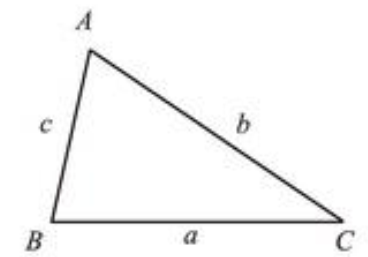
\includegraphics[width=0.3\linewidth]{pic/20200425013.png}
    \item 构成:三角形有三条边,三个角和三个顶点.
    \item 符号表示:三角形用符号\(\triangle \)表示.\(\triangle ABC\)的三个角可以用\(\angle A, \angle B, \angle C\)表示,三边有时也用a, b, c表示.大小写字母\tkt{相对}.
    \end{zsyd}
\item 三角形的分类\\
    \begin{zsyd}
    \item 按角度\tkt{\(\begin{cases} \text{斜三角形}\begin{cases} \text{锐角三角形}\\ \text{钝角三角形} \end{cases}\\ \text{直角三角形} \end{cases}\)}\\
        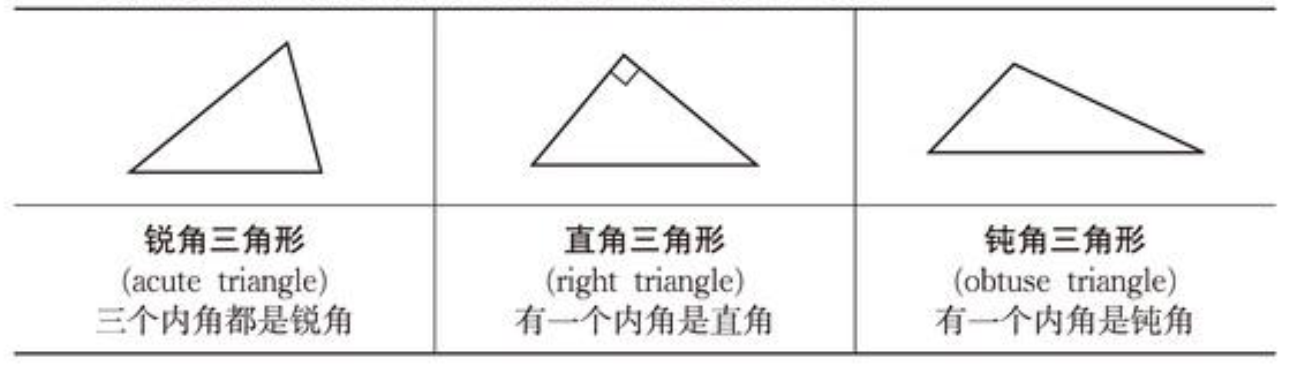
\includegraphics[width=0.6\linewidth]{pic/20200425014.png}
        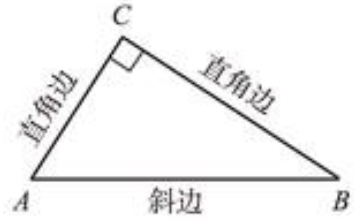
\includegraphics[width=0.3\linewidth]{pic/20200425015.png}\\
    \item 按边的关系:\tkt{\(\begin{cases} \text{三标都不相等的三角形}\\ \text{等腰三角形}\begin{cases} \text{底边和腰不相等的等腰三角形}\\ \text{等边三角形}\end{cases} \end{cases}\)}\\
        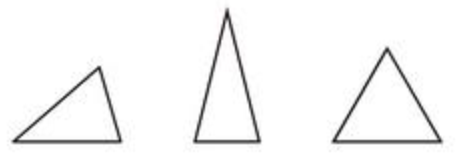
\includegraphics[width=0.6\linewidth]{pic/20200425016.png}
        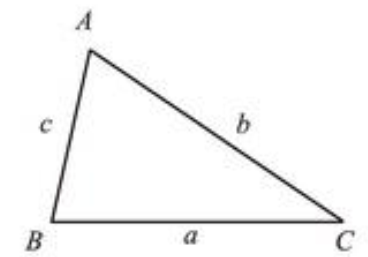
\includegraphics[width=0.3\linewidth]{pic/20200425013.png}
    \end{zsyd}
\item 三角形的性质
    \begin{zsyd}
    \item 普遍性质
        \begin{zsyd}
        \item 稳定性
        \item 三角形\tkt{\(\text{三个内角的和等于}180^\circ\)}
        \item 三角形\tkt{任意两边之和大于第三边}
        \item 三角形\tkt{任意两边之差小于第三边}
        \end{zsyd}
    \item 特殊三角形的特有性质
        \begin{zsyd}
        \item 直角三角形的\tkt{两个锐角互余}
        \item 等腰直角三角形的三个角为:\tkt{\(90 ^\circ, 45^\circ, 45^\circ\)}
        \item 等边三角形的\tkt{三条边相等},三个角都是\tkt{\(60 ^\circ\)}
        \item 同一个三角形中,等边对\tkt{等角},\tkt{等角}对等边
        \end{zsyd}
    \end{zsyd}
\item 三角形中的重要线段:三线和中位线
    \begin{zsyd}
    \item 中线
        \begin{zsyd}
        \item 定义:如图,三角形中\tkt{连接一个顶点与它对边中点的线段},叫做这个三角形的中线(median).\\
            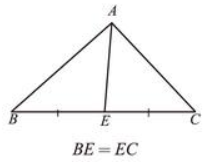
\includegraphics[width=0.3\linewidth]{pic/20200425018.png}
        \item 性质:中线\tkt{将三角形分成两个面积相等的小三角形}.
        \item 交点:三角形三条中线\tkt{交于一点},这点称为三角形的\tkt{\textbf{重心}}.
        \end{zsyd}
    \item 角平分线
        \begin{zsyd}
        \item 定义:如图,三角形中,一个内角的角平分线与它的对边相交,这个角的顶点与交点之间的线段叫做三角形的角平分线.\\
            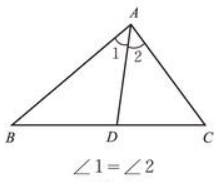
\includegraphics[width=0.3\linewidth]{pic/20200425019.png}
        \item 性质:角平分线上\tkt{的点到角的两边的距离相等}(\tkt{从点向两边作垂线段}).
        \item 交点:三角形三条角平分线\tkt{交于一点},这点称为三角形的\tkt{\textbf{内心}}.
        \end{zsyd}
    \item 高
        \begin{zsyd}
        \item 定义:如图,从三角形的\tkt{一个顶点向它的对边所在直线作垂线,顶点和垂足之间}的线段叫做三角形的高线,简称三角形的高(height).\\
            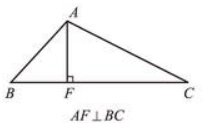
\includegraphics[width=0.3\linewidth]{pic/20200425020.png}
        \item 性质:高可能在三角形内(\tkt{锐角}三角形),可能在三角形外(\tkt{钝角}三角形),也可能与边重合(\tkt{直角}三角形).
        \item 交点:三角形三条角平分线交于\tkt{一点},这点称为三角形的\tkt{\textbf{内心}}.
        \end{zsyd}
    \item 中位线
        \begin{zsyd}
        \item 定义:连接三角形\tkt{两边中点}的线段叫做三角形的中位线
        \item 性质:三角形的中位线\tkt{平行于第三边并等于第三边的一半}
        \item 用法:(1)遇到三角形中点时, 常构造三角形的中位线,证明\tkt{线段平行或倍分}问题,可简单的概括为``\tkt{已知中点找中位线}''; (2)在平行四边形或特殊的平行四边形中遇到边上中点时,可连接中点与\tkt{对角线的交点}构造中位线
        \end{zsyd}
    \end{zsyd}
\item 三角形的四心
    \begin{zsyd}
    \item 内心:\tkt{三条角平分线的交点}
    \item 外心:\tkt{三条中垂线的交点}
    \item 重心:\tkt{三条中线的交点}
    \item 垂心:\tkt{三条高的交点}\\
        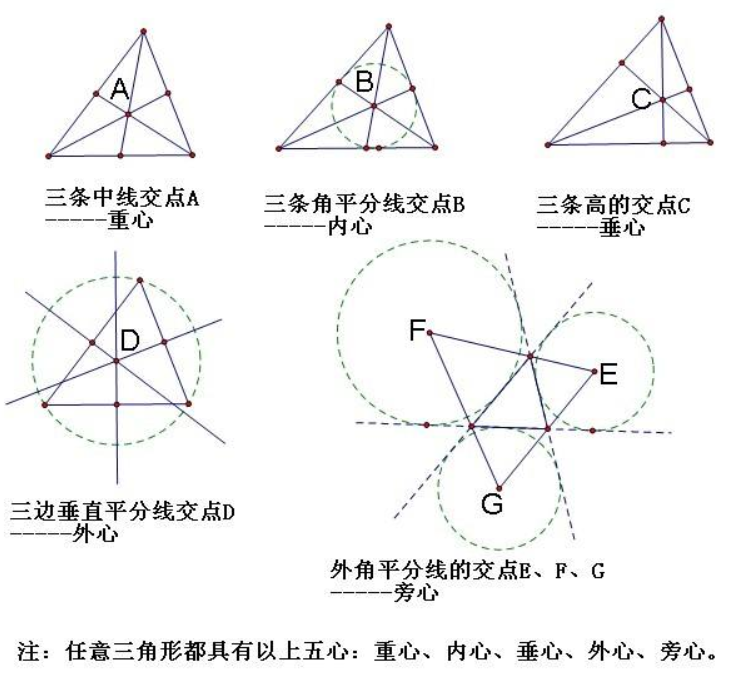
\includegraphics[width=0.5\linewidth]{pic/20200426001.png}
    \end{zsyd}
\item 三角形的外角
    \begin{zsyd}
    \item 定义:三角形的外角是三角形的一边与另一边的\tkt{反向延长线}组成的角.\\
        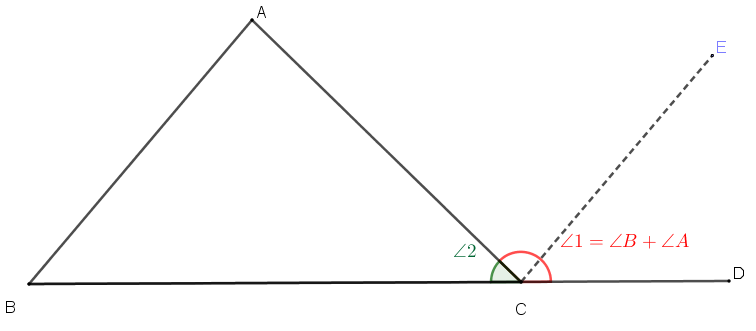
\includegraphics[width=0.5\linewidth]{pic/20200427003.png}
    \item 性质
        \begin{zsyd}
        \item 三角形的一个外角等于\tkt{不相邻的两个内角和}
        \item 三角形的一个外角大于\tkt{与它不相邻的任一内角}
        \item 三角形三个外角之和为\tkt{\(360 ^\circ\)}
        \item 三角形的每个顶点处都有\tkt{两个相等}的外角,所以每个三角形都有\tkt{六个}外角
        \end{zsyd}
    \end{zsyd}
\begin{note}
        习题4.29
\end{note}
\end{zsyd}
\chapter{专题:截长补短法}%
\label{cha:专题:截长补短法}
适用:当已知或求证中涉及线段的和(或差)等于另一条线段(或几条线段的和或差)时.
\begin{liti}
\item 如图,在\(\triangle ABC\)中, \(\triangle C = 2\triangle B, \triangle 1 = \triangle 2\).求证: \(AB=AC + AC+CD\)\\
    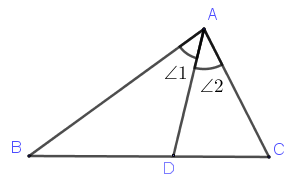
\includegraphics[width=0.4\linewidth]{pic/20200513001.png}\\
    解一:截长法:在AB上截取\(AE = AC\).\\
    解二:补短法:延长AC到E使\(CF=CD\).
\begin{solution}
        一. 截长法:\\
        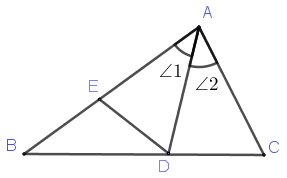
\includegraphics[width=0.4\linewidth]{pic/20200513002.png}\\
        证:\(\begin{cases} AE=AC\\ \angle 1 = \angle 2\\ AD=AD \end{cases} \Rightarrow \triangle AED \cong \triangle ACD (SAS) \Rightarrow \angle AED = \angle C , DE=CD\)\\
        \(\begin{cases} \angle AED = \angle C= 2\angle B\\ AED = \angle B + \angle EDB (\text{外角})\\  \end{cases} \Rightarrow \angle B = \angle EDB \Rightarrow BE=DE=CD\)\\
        \(\begin{cases} AE=AC\\ BE=DE=CD\\ AB=AE+BE \end{cases}\Rightarrow AB=AC+CD\)
        \(\therefore \)得证.\\
        二. 补短法\\
        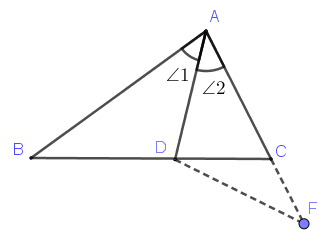
\includegraphics[width=0.4\linewidth]{pic/20200513003.png}\\
        证:如图,延长\(AC\)到\(F\),使\(CF=CD\)\\
        \(\begin{cases} CD=CF \Rightarrow \angle F = \angle CDF\\ \angle ACD=\angle CDF + \angle F \\ \angle ACD = 2\angle B \end{cases} \Rightarrow \angle B = \angle F\)\\
        \(\begin{cases} \angle B = \angle F\\ \angle 1 = \angle 2\\ AD=AD \end{cases} \Rightarrow \triangle ADB \cong \triangle ADF \Rightarrow AB=AF\)\\
        \(\begin{cases} AB=AF\\ CD = CF\\ AF=AC+CF \end{cases}\Rightarrow AB=AC+CD\)\\
        \(\therefore \)得证.
\end{solution}
\end{liti}
\begin{shiti}
\item 如图,在正方形\(ABCD\)中,\(E\)为\(BC\)上的一点,\(F\)为\(CD\)上的一点,\(BE + DF = EF\),则\(\angle EAF\)的度数为(\qquad)\\
    \begin{tasks}(4)
        \task \(30 ^\circ\)
        \task \(37.5 ^\circ\)
        \task \(45 ^\circ\)
        \task \(60 ^\circ\)
    \end{tasks}
\item 如图, 已知\(AD // BC,AB = AD + BC\),\(E\)是\(CD\)的中点,则\(\angle AEB\)的度数为\tkt{\qquad}.
\item 如图,\(\triangle ABC\)中, \(\triangle CAB = \triangle CBA =45^\circ\),点\(E\)为\(BC\)的中点,\(CN \perp AE\)交\(AB\)于点\(N\).求证\(AE=CN+EN\).
\end{shiti}

\chapter{全等三角形}%
\label{cha:全等三角形}
\begin{note}
    【对接教材】 人教:八上第十二章P30-P56;北师: 七下第四章P92-P104.P108-P113
\end{note}
\begin{zsyd}
\item 全等三角形的判定
    \begin{zsyd}
    \item 一般三角形的判定
        \begin{zsyd}
        \item \tkt{SSS(边边边)}: \tkt{三边分别相等的两个三角形全等}
        \item \tkt{SAS(边角边)}: \tkt{两边和它们的夹角分别相等的两个三角形全等}
        \item \tkt{ASA(角边角)}: \tkt{两角和它们的夹边分别相等的两个三角形全等}
        \item \tkt{AAS(角角边)}: \tkt{两边和其中一个角的对边分别相等的两个三角形全等}
        \end{zsyd}
    \item 直角三角形的判定\\
        \tkt{HL}:\tkt{斜边和一条直角边分别相等的两个直角三角形全等}
    \item 【易错警示】
        \begin{zsyd}
        \item ``HL''只适用于\tkt{直角三角形全等}的判定;
        \item \tkt{``SSA''},\tkt{''AAA''}不能判定三角形全等;
        \item 证明三角形全等时, \tkt{对应顶点的字母必须写在对应位置上}
        \end{zsyd}
    \end{zsyd}
\item 全等三角形的性质
    \begin{zsyd}
    \item 全等三角形的对应边 \tkt{相等},对应角\tkt{相等}
    \item 全等三角形的对应线段(\tkt{角平分线},\tkt{中线},\tkt{高线},\tkt{中位线})相等,对应\tkt{周长}相等,对应\tkt{面积}相等
    \end{zsyd}
\item 判定两个三角形全等的思路
    \begin{zsyd}
    \item  已知两组边
        \begin{zsyd}
        \item 找\tkt{夹角}: \tkt{SAS}
        \item 找\tkt{直角}: \tkt{HL}
        \item 找\tkt{第三边}: \tkt{SSS}
        \end{zsyd}
    \item  已知一组边和一组角
        \begin{zsyd}
        \item 边为角的对边\(\to\)找\tkt{任意一角}\(\to\)\tkt{AAS}
        \item 边为角的邻边\(\to \)\(\begin{cases} \text{找\tkt{夹角的另一边}}\to\tkt{SAS}\\ \text{找\tkt{夹边的另一角}}\to\tkt{ASA}\\ \text{找\tkt{边的对角}}\to\tkt{AAS} \end{cases}\)
        \end{zsyd}
    \item  已知两角
        \begin{zsyd}
        \item 找\tkt{夹边} \(\to \) \tkt{ASA}
        \item 找\tkt{其中一角的对边}\(\to \)\tkt{AAS}
        \end{zsyd}
    \end{zsyd}
\item 常考全等模型
    \begin{zsyd}
    \item 平移型
        \begin{zsyd}
        \item 模型示例\\
            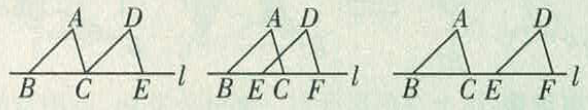
\includegraphics[width=0.8\linewidth]{pic/20200511001.png}
        \item 模型分析\\
            此模型特征是有一组边共线或部分重合,另两组边分别平行,常要在\tkt{移动方向上加(减)公共线段},构造线段相等,或利用\tkt{平行线性质}找到对应角相等.
        \end{zsyd}
    \item 轴对称型
        \begin{zsyd}
        \item 模型示例\\
            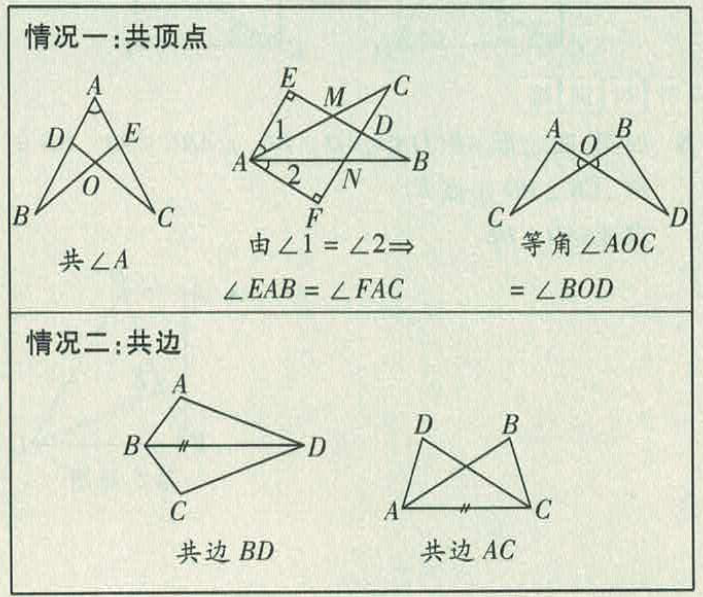
\includegraphics[width=0.8\linewidth]{pic/20200511002.png}
        \item 模型分析:此模型的特征是所给图形可沿某一直线折叠,直线两旁的部分能完全重合,重合的顶点就是全等三角形的对应顶点,解题时要注意其隐含条件,即\tkt{公共边或公共角相等}.
        \end{zsyd}
    \item 一线三垂直型
        \begin{zsyd}
        \item 模型示例\\
            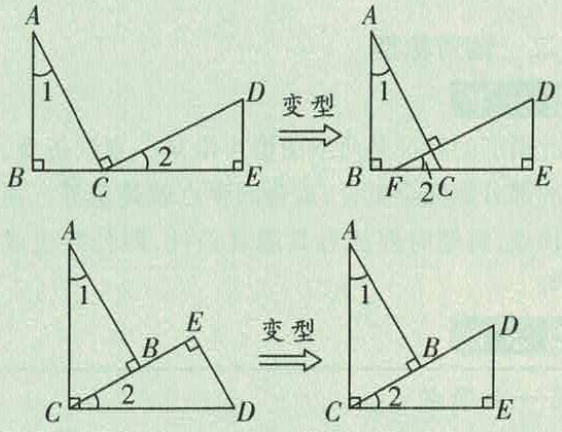
\includegraphics[width=0.8\linewidth]{pic/20200511003.png}
        \item 模型分析\\
            一线:\tkt{经过直角顶点的直线};三垂直:\tkt{直角两边互相垂直},\tkt{过直角的两边向直线作垂直},利用``\tkt{同角的余角相等}''转化找等角\tkt{\(\angle 1 = \angle 2\)}
        \end{zsyd}
    \item 旋转型:此模型可看成是将三角形绕着公共顶点旋转一定角度所构成的,旋转后的图形与原图之间存在两种情况
        \begin{zsyd}
        \item 无重叠旋转型
            \begin{zsyd}
            \item 模型示例\\
                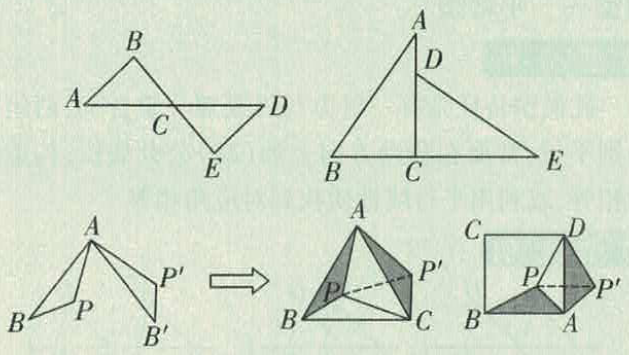
\includegraphics[width=0.8\linewidth]{pic/20200511004.png}
            \item 模型分析\\
                两个三角形有公共顶点,无重叠部分.一般\tkt{一对隐含的等角}(通过\tkt{对顶角相等}或\tkt{平行线}性质得到)
            \end{zsyd}
        \item 有重叠旋转型
            \begin{zsyd}
            \item 模型示例\\
                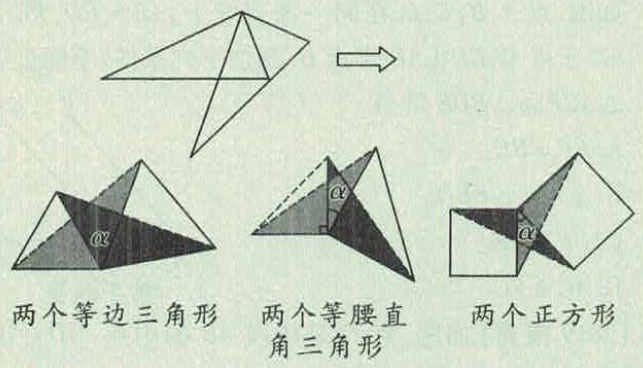
\includegraphics[width=0.8\linewidth]{pic/20200511005.png}\\
            \item 模型分析\\
                两个三角形含有一部分\tkt{公共角},运用\tkt{角的和差}可得到的等角
            \end{zsyd}
        \end{zsyd}
    \end{zsyd}
\end{zsyd}

\chapter{等腰三角形与直角三角形}%
\label{cha:等腰三角形与直角三角形}

\section{知识要点}%
\label{sec:知识要点}

\begin{zsyd}
\item 等腰三角形与等边三角形
    \begin{table}[H]
        \centering
        \caption{等腰三角形与等边三角形对比}
        \begin{tabular}{|c|p{16em}|p{16em}|}
            \hline
          & \multicolumn{1}{c|}{\textbf{等腰三角形}} & \multicolumn{1}{c|}{\textbf{等边三角形}} \bigstrut\\
          \hline
            \textbf{定义} & \tkt{至少有两边}相等的三角形.相等的两个边称为这个三角形的腰。 & 三边相等的三角形 \bigstrut\\
            \hline
            \multirow{3}[6]{*}{\textbf{性质}} & \tkt{两腰}相等,\tkt{两底角}相等 & 三条边相等,三个角相等,均为\tkt{\(60 ^\circ\)} \bigstrut\\
            \cline{2-3}          & \tkt{顶角平分线},\tkt{底边上的中线},\tkt{底边上的高}相互重合 & \tkt{同一条边上的任意三线}重合 \bigstrut\\
            \cline{2-3}          & 是\tkt{轴对称}图形,有\tkt{一条对称}轴 & 有\tkt{三条对称轴} \bigstrut\\
            \hline
            \multirow{2}[4]{*}{\textbf{判定}} & 两边相等的三角形是等腰三角形 & 三边相等的三角形是等边三角形 \bigstrut\\
            \cline{2-3}          & 两个角相等的三角形是等腰三角形 & \multicolumn{1}{p{21.165em}|}{(1)三个角相等的三角形是等边三角形\newline{}(2)有一个角是\tkt{\(60 ^\circ\)}的\tkt{等腰三角形}是等边三角形} \bigstrut\\
            \hline
            \textbf{面积} & \(S=\)\tkt{\(\frac{1}{2}ah\)}(\(h\)是底边\(a\)上的高)   & \(S\)=\(\frac{1}{2}ah\)=\tkt{\(\frac{\sqrt{3}}{4}a^2\)}(\(h\)是任意边\(a\)上的高) \bigstrut\\
            \hline
        \end{tabular}%
        \label{tab:addlabel}%
    \end{table}%
    【技巧】 (1)等腰三角形中求角度: 当已知等腰三角形的一个角时, 要\tkt{先确定该角是顶角还是底角}, 再分情况进行讨论;\\
    (2)等腰三角形中求边:当已知等腰三角形两边时,除了要\tkt{确定哪条边作为腰或底}外,还要考虑\tkt{三角形三边关系}这个前提条件
\item 直角三角形
    \begin{zsyd}
    \item 定义:有一个角为直角的三角形.
    \item 分类\tkt{\(\begin{cases} \text{特殊直角三角形} \begin{cases} \text{等腰直角三角形}\\ 30^\circ\text{和}60^\circ\text{直角三角形}\\  \end{cases}\\ \text{普通直角三角形} \\  \end{cases}\)}
    \item 性质
        \begin{zsyd}
        \item 两锐角之和等于\tkt{\(90^\circ\)}
        \item 斜边上的中线等于 \tkt{斜边的一半}
        \item  \(30 ^\circ\)角所对的直角边等于 \tkt{斜边的一半}
        \item 若一条直角边\tkt{等于斜边的一半}, 则这条直角边所对的锐角等于 \tkt{\(30 ^\circ\)}
        \item 勾股定理:若直角三角形的两直角边长分别为\(a, b\),斜边长为\(c\),则有\tkt{\(a^2+b^2=c^2\)}
        \item \(S =\) \tkt{\(\frac{1}{2}ab\)}=  \tkt{\(\frac{1}{2}ch\)}  ( \(a, b\)为两个直角边,\(h\)为斜边\(c\)上的高)
        \end{zsyd}
    \item 判定
        \begin{zsyd}
        \item 有一个角为 \tkt{\(90 ^\circ\)}的三角形是直角三角形
        \item 勾股定理逆定理:如果三角形的三边长分别为\(a, b, c\),若满足  \tkt{\(a^2+b^2=c^2\)} , 那么这个三角形是直角三角形
        \item 有两个角\tkt{互余}的三角形是直角三角形
        \item 一条边上的 \tkt{中线}等于这条边的一半的三角形是直角三角形(应用时需先证明)
        \end{zsyd}
    \end{zsyd}
\item 等腰直角三角形
    \begin{zsyd}
    \item 定义:\tkt{两直角边相等}的直角三角形.
    \item 性质
        \begin{zsyd}
        \item 具有直角三角形的所有性质(\tkt{两锐角和},\tkt{斜边中线},\tkt{勾股定理},面积公式)
        \item \tkt{两直角边相等}
        \item 两锐角相等且都等于\tkt{\(45 ^\circ\)}
        \item 面积:\(S=\)\tkt{\(\frac{1}{2}a^2\)}=\tkt{\(\frac{1}{2}ch\)}=\tkt{\(\frac{1}{4}c^2\)}=\tkt{\(\frac{\sqrt{2}}{2}ah\)},其中\(a\)为直角边,\(h\)为斜边\(c\)上的高(\(c=\sqrt{2}a\))
        \end{zsyd}
    \item 判定
        \begin{zsyd}
        \item 顶角为 \tkt{\(90 ^\circ\)}的等腰三角形是等腰直角三角形
        \item 有两个角为 \tkt{\(45 ^\circ\)}的三角形是等腰直角三角形
        \item 有一个角为\tkt{\(45^\circ\)}的 \tkt{直角}三角形是等腰直角三角形
        \item \tkt{两条直角边}相等的直角三角形是等腰直角三角形
        \end{zsyd}
    \end{zsyd}
\end{zsyd}
\chapter{中点问题六种方法}%
\label{cha:中点问题六种方法}

\begin{zsyd}
\item 方法汇总
    \begin{enumerate}
        \item 中点或平行+中点\(\to \)\tkt{构造中位线};
        \item 角+斜边中点\(\to \)\tkt{直角三角形斜边中线};
        \item 中线或与中点有关线段\(\to \)\tkt{倍长线段构造全等};
        \item 等腰+底边中点\(\to \)\tkt{等腰三角形三线合一};
        \item 同一边遇垂直+中点\(\to \)\tkt{垂直平分线性质}
    \end{enumerate}
\item 见三角形边上的中点,构造中位线
    \begin{zsyd}
    \item 场景: (1)已知点D,E分别为AB,AC的中点; (2)已知点D为AB的中点\\
        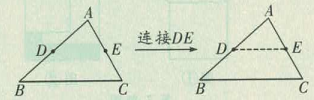
\includegraphics[width=0.3\linewidth]{pic/20200512001.png}
        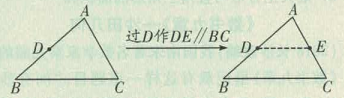
\includegraphics[width=0.3\linewidth]{pic/20200512002.png}
    \item 结论:\tkt{\(DE // BC\)} , \tkt{\(DE = \frac{1}{2}BC\)}
    \item 用途:证明\(\triangle ADE \sim \triangle ABC\),解决线段之间的相等或比例关系及平行问题.
    \end{zsyd}
\item 见直角三角形斜边上的中点, 构造中线
    \begin{zsyd}
    \item 场景: 已知,\(Rt\triangle ABC,\triangle C=90 ^\circ\),点\(D\)为\(AB\)的中点.\\
        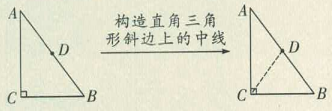
\includegraphics[width=0.5\linewidth]{pic/20200512003.png}\\
        注:有时有直角, 无中点, 可以找斜边中点, 构造斜边
    \item 结论: \tkt{\(CD=AD=BD\frac{1}{2}AB\)}, \tkt{\(\triangle ACD,\triangle BCD\)都是等腰三角形}
    \item 用途: \ding{172}证明线段相等或求线段长; \ding{173}构造角相等进行等量代换.
    \end{zsyd}
\item 遇到三角形一边上的中点, 考虑倍长中线,
    \begin{zsyd}
    \item 场景\\
        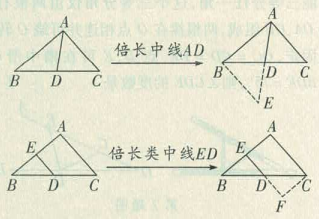
\includegraphics[width=0.3\linewidth]{pic/20200512004.png}
    \item 结论: \tkt{\(\triangle ADC \cong \triangle EDB\)} ; \tkt{\(\triangle BED \cong \triangle CFD\)};
    \item 用途:构造全等三角形, 证明线段间的数量关系.
    \end{zsyd}
\item 见等腰三角形底边上的中点作中线,构造``三线合一''
    \begin{zsyd}
    \item 场景:已知,点\(D\)为\(\triangle ABC\)边\(BC\)的中点\\
        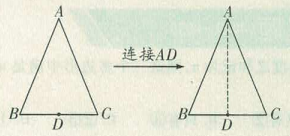
\includegraphics[width=0.3\linewidth]{pic/20200512005.png}\\
        注:有等腰三角形,无中点,可以找底边中点构造``三线合一''
    \item 结论:\tkt{\(BD=CD\)};\tkt{\(\angle BAD=\angle CAD\)}; \tkt{\(AD \perp BC\)}
    \item 用途:解决线段相等及垂直问题,角度转化及相等问题
    \end{zsyd}
\item 见垂直平分线,构造等腰三角形
    \begin{zsyd}
    \item 场景:已知,在\(\triangle ABC\)中,\(ED\)垂直平分\(BC\).\\
        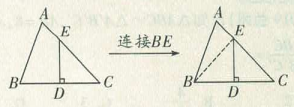
\includegraphics[width=0.3\linewidth]{pic/20200512006.png}
    \item 结论:\tkt{\(BE=CE\)};\tkt{\(BD=CD\)}
    \item 用途:证明线段间的数量关系
    \end{zsyd}
\item 中线平分三角形面积
    \begin{zsyd}
    \item 场景:已知,AD是\(\triangle ABC\)的中线\\
        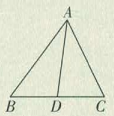
\includegraphics[width=0.2\linewidth]{pic/20200512007.png}
    \item 结论: \(S_{\triangle ABD}=\)\tkt{\(S_{\triangle ACD}\)}\(=\)\tkt{\(\frac{1}{2}\)}\(S_{\triangle ABC}\)
    \item 用途:证明三角形面积间数量关系
    \end{zsyd}
\end{zsyd}
\chapter{相似三角形及其应用}%
\begin{note}
    【对接教材】 人教: 九下第二十七章P23-P46; 北师: 九上第四章P75 -P112.
\end{note}
\section{知识要点}%
\label{sec:知识要点}

\begin{zsyd}
\item 预备知识:比与比例\\
    \begin{table}[H]
        \centering
        \caption{比与比例}
        \begin{tabular}{|l|p{16em}|p{16em}|}
            \hline
          & \textbf{比} & \textbf{比例} \bigstrut\\
          \hline
            定义 & 两个数\tkt{相除}又叫做两个数的比 & 表示\tkt{两个比相等的式子}叫做比例 \bigstrut\\
            \hline
            各部分名称 & 前项:后项=比值\newline{}90:60=1.5 & 外项,内项\newline{}9:6=3:2 \bigstrut\\
            \hline
            基本性质 & 比的前项和后项\tkt{同时乘或除一个不为0的数},比值不变 & \tkt{两个外项的积等于两个内项的积} \bigstrut\\
            \hline
            常用运算  & 化简比   & 解比例(\tkt{求比例中的一个未知项}) \bigstrut\\
            \hline
        \end{tabular}%
        \label{tab:addlabel}%
    \end{table}%
\item 比例线段
    \begin{zsyd}
    \item 比例性质
        \begin{zsyd}
        \item \tkt{\(\frac{a}{b}=\frac{c}{d}\iff ad=bc (abcd\ne 0)\)}
        \item 合比性质: 如果\(\frac{a}{b}=\frac{c}{d}\),那么\(\frac{a\pm b}{b}=\)\tkt{\(\frac{c\pm d}{d}\)}
        \item 等比性质: 如果\(\frac{a}{b}=\frac{c}{d}=\cdots =\frac{m}{n} (b+d+\cdots+n)\ne 0\),那么 \(\frac{a + c + \cdots +m}{b + d + \cdots+n} = \) \tkt{\(\frac{a}{b}\)}
        \end{zsyd}
    \item 黄金分割:一般地,如图\ding{172}, 点\(C\)把线段\(AB\)分成两条线段\(AC\)和\(BC\),如果\tkt{\(\frac{AC}{AB}=\frac{BC}{AC}\)},那么称线段AB被点C黄金分割, 点C叫做线段AB的黄金分割点,AC与AB的比叫黄金比,即第\(\frac{AC}{AB}=\)\tkt{\(\frac{\sqrt{5}-1}{2} \)}\(\approx\) \tkt{\(0.618\)}\\
        \includegraphics[width=0.15\linewidth]{pic/20200514001.png}
    \item 平行线分线段成比例
        \begin{zsyd}
        \item 基本事实:两条直线被一组平行线所截,所得的\tkt{对应线段成比例}, 如图\ding{173}. 当\(l_3 // l_4 //l_5\)时, 有\(\frac{AB}{BC}=\)\tkt{\(\frac{DE}{EF}\)}, \(\frac{AB}{AC}=\)\tkt{\(\frac{DE}{DF}\)}等.\\
        \includegraphics[width=0.25\linewidth]{pic/20200514002.png}
    \item 推论:平行于三角形一边的直线截其他两边(或两边的延长线),所得的\tkt{对应线段成比例}, 如图\ding{174},当\(DE//BC\)时, 有\(\frac{AD}{DB}=\)\tkt{\(\frac{AE}{EC}\)},\(\frac{AD}{AB}=\)\tkt{\(\frac{AE}{AC}\)}\(=\)\tkt{\(\frac{DE}{BC}\)}\\
        \includegraphics[width=0.15\linewidth]{pic/20200514003.png}\\
        \end{zsyd}
    \end{zsyd}
\item 相似三角形的性质
    \begin{zsyd}
    \item 相似三角形对应角\tkt{相等},对应边\tkt{成比例}.
    \item 相似三角形的对应线段(\tkt{边},\tkt{高},\tkt{中线},\tkt{角平分线})成比例,且等于\tkt{相似比}
    \item 相似三角形的周长比\tkt{等于相似比}, 面积比 \tkt{等于相似比的平方}
    \end{zsyd}
\item 相似三角形的判定
    \begin{zsyd}
    \item \tkt{AA}:\tkt{两角}对应\tkt{相等}, 两三角形相似
    \item \tkt{SAS}:\tkt{两边}对应\tkt{成比例}, 且\tkt{夹角}相等,两三角形相似
    \item \tkt{AAA}:三边对应\tkt{成比例} ,两三角形相似
    \item \tkt{平行于三角形一边}的直线和\tkt{其他两边或两边的延长线}所构成的三角形与原三角形相似
    \end{zsyd}

\item 相似三角形的判定思路
    \begin{zsyd}
    \item 有平行截线\(\to \)用\tkt{平行线的性质找等角}
    \item 有一对等角\(\to \)找\tkt{另一对等角或该角的两边对应成比例}
    \item 有两组边对应成比例\(\to \)找\tkt{夹角相等}或\tkt{第三边对应成比例}
    \item 直角三角形\(\to \)找\tkt{一对锐角相等}或\tkt{两条边对应成比例}
    \item 等腰三角形\(\to \)找\tkt{顶角相等}或\tkt{一对底角}相等
    \end{zsyd}

\item 相似三角形的实际应用
    \begin{zsyd}
    \item 运用相似三角形的判定条件和性质解决实际问题的方法步骤
        \begin{zsyd}
        \item 将实际问题转化为相似三角形问题
        \item 找出一对相似三角形
        \item 根据相似三角形的性质, 表示出相应的量\tkt{列比例式}求解
        \end{zsyd}
    \item 相似三角形的几种实际应用类型
        \begin{zsyd}
        \item 测量高度:测量不能达到顶部的物体的高度, 通常使用``\tkt{在同一时刻物高与影长成比例}''
        \item 测量距离:测量不能直接到达的两点间的距离, 常\tkt{构造相似三角形}求解
        \end{zsyd}
    \end{zsyd}
\end{zsyd}

\chapter{常考相似模型}%
\label{cha:常考相似模型}
\section{知识要点}%
\label{sec:知识要点}

\begin{zsyd}
\item A字型
    \begin{zsyd}
    \item 模型分析\\

        \includegraphics[width=0.9\linewidth]{pic/20200514004.png}\\
        有一个公共角(\(\angle A)\)或有公共顶点的一对等角(图\ding{172}:\(\angle BAC =\angle DAE\)), 此时需要\tkt{找另一对角相等}.若题中未明确相似三角形对应顶点, 则需要分类讨论, 如图\ding{172}中可找条件\tkt{\(\angle ADE = \angle B\)},图\ding{173}可找条件\tkt{\(\angle ADE=\angle C\)}.
    \item 结论
        \begin{zsyd}
        \item 图\ding{175},图\ding{176}:\tkt{\(AC^2 =AD\cdot AB\)}
        \item 图\ding{176}:\ding{172}\tkt{\(CD^2=AD\cdot BD\)}; \ding{173}\tkt{\(BC^2 =BD\cdot AB\)}
        \end{zsyd}
    \item 例题
    \end{zsyd}
    \begin{liti}
    \item 如图, 在\(\triangle ABC\)中, 点\(D,E\)分别在\(AB,AC\)边上,\(DE // BC\) ,若\(AD=1 ,BD=2\),则\(\frac{DE}{BC}\)的值为(\qquad)\\
        \includegraphics[width=0.2\linewidth]{pic/20200514005.png}\\
        \begin{tasks}(4)
            \task \(\frac{1}{2}\)
            \task \(\frac{1}{3}\)
            \task \(\frac{1}{4}\)
            \task \(\frac{1}{9}\)
        \end{tasks}
\begin{solution}
            B.\(\frac{DE}{BC}=\frac{AD}{AD+BD}\)\\
\end{solution}
    \item  如图,\(D,E\)分别是 \(\triangle ABC\)边\(AB, AC\)上的点, \(\angle ADE=\angle ACB\),若\( AD = 2,AB =6,AC=4\),则 \(AE\)的长是(\qquad)\\
        \includegraphics[width=0.3\linewidth]{pic/20200514006.png}\\
        \begin{tasks}(4)
            \task \(1\)
            \task \(2\)
            \task \(3\)
            \task \(4\)
        \end{tasks}
    \end{liti}
\item 8字型
    \begin{zsyd}
    \item 模型分析\\
        \includegraphics[width=0.5\linewidth]{pic/20200514007.png}\\
        有一组隐含的\tkt{等角(对顶角)},此时需要从已知条件中、\tkt{图中隐含条件}或通过证明得\tkt{另一对角相等}.若题中未明确相似三角形对应顶点, 则需要分类讨论
    \item 结论
    \item 例题
    \end{zsyd}
    \begin{liti}[resume]
    \item 如图, 把一张三角形纸片\(ABC\)沿中位线\(DE\)剪开后, 在平面上将绕着点\(E\)顺时针旋转\(180 ^\circ\) ,点\(D\)到了点\(F\)的位置, 则\(S_{\triangle ADE}:S_{\parallelogram BCFD}=\)(\qquad)\\
        \includegraphics[width=0.2\linewidth]{pic/20200514008.png}\\
        \begin{tasks}(4)
            \task  \(1:3\)
            \task  \(1:1\)
            \task  \(1:4\)
            \task  \(1:2\)
        \end{tasks}
\begin{solution}
            D\\
\end{solution}
    \end{liti}
\item 一线三等角型(K型)
    \begin{zsyd}
    \item 模型分析\\
        常以等腰三角形或等边三角形为背景, 三个等角顶点在同一直线上, 称一线三等角模型, 其中\(\angle 1 = \angle 2 =\angle 3\),可根据三角形内角和及补角得到另一组等角.可得下面三个图形中\tkt{两阴影部分三角形}相似.\\
        \includegraphics[width=0.8\linewidth]{pic/20200514009.png}\\
        \includegraphics[width=0.8\linewidth]{pic/20200514010.png}\\
    \item 一线三直角常存在的图形背景\\
        \includegraphics[width=0.2\linewidth]{pic/20200514011.png}
        \includegraphics[width=0.2\linewidth]{pic/20200514012.png}
        \includegraphics[width=0.2\linewidth]{pic/20200514013.png}
        \includegraphics[width=0.2\linewidth]{pic/20200514014.png}
    \end{zsyd}
    \begin{liti}[resume]
    \item 如图, 在\(\triangle ABC\)中,\(AB=AC\),点\(P,D\)分别是\(BC,AC\)边点上的点, 且\(\angle APD= \angle B\),求证:\(AC \cdot  CD = CP \cdot BP\).\\
        \includegraphics[width=0.2\linewidth]{pic/20200514015.png}
\begin{solution}
            \(AB=AC \Rightarrow \angle B=\angle C \Rightarrow \angle APD = \angle B=\angle C \)\\
            \(\begin{cases} \angle APC = \angle APD + \angle DPC\\ \angle APC = \angle B + \angle BAP\\ \angle APD =\angle B \end{cases}\angle BAP = \angle DPC\)\\
            \(\begin{cases} \angle BAP = \angle DPC\\ \angle B = \angle C \end{cases} \Rightarrow \triangle ABP \sim \triangle PCD \Rightarrow \frac{BP}{AB}=\frac{CD}{CP}\)\\
            \(\frac{BP}{AB}=\frac{CD}{CP},\text{且}AB=AC \Rightarrow \frac{BP}{AC}=\frac{CD}{CP}\Rightarrow AC\cdot CD = CP\cdot BP\)
\end{solution}

    \item 如图, 在正方形\(ABCD\)中, 点\(E,F,G\)分别在\(AB,BC,CD\) 上, 且\(\angle EFG = 90 ^\circ\).若 \(AB = 12,AE = 3,CF=4\)求\(CG\)的长.\\
        \includegraphics[width=0.2\linewidth]{pic/20200514016.png}\\
\begin{solution}
            \(\angle EFB + \angle GFC = 90^\circ \Rightarrow \angle BEF = \angle CGF \Rightarrow Rt\triangle BEF \sim Rt\triangle CGF \Rightarrow \frac{CG}{CF}=\frac{BF}{BE}\)\\
            \(AB =12, AE=3,CF=4 \Rightarrow BE = 9, BF=8 \Rightarrow \frac{CG}{4}=\frac{8}{9}\Rightarrow CG = \frac{32}{9}\)
\end{solution}
    \end{liti}
\end{zsyd}

\chapter{锐角三角函数及其应用}%
\label{cha:锐角三角函数及其应用}
\begin{note}
    【对接教材】 人教: 八下第十七章P21 - P39,九下第二十八章P60 - P85; 北师: 九下第一章P】-P27.
\end{note}
\begin{zsyd}
\item 三角函数定义\\
    如图,\(Rt\triangle ABC中,\angle C=90 ^\circ, \angle A, \angle B, \angle C\)的对边分别为\(a,b,c\)\\
    \includegraphics[width=0.2\linewidth]{pic/20200511006.png}
    \begin{zsyd}
    \item \(\angle A\)的正弦: \(\sin A =\) \tkt{\(\frac{\angle A\text{的对边}}{\text{斜边}}\)}\(=\)\tkt{\(\frac{a}{c}\)}
    \item \(\angle A\)的余弦: \(\cos A = \frac{\angle A\text{的邻边}}{\text{斜边}}=\)\tkt{\(\frac{b}{c}\)}
    \item \(\angle A\)的正弦: \(\tan A =\) \tkt{\(\frac{\angle A\text{的对边}}{\angle A\text{的邻边}}\)}\(=\)\tkt{\(=\qquad\)}
    \item 【技巧】三角函数是在直角三角形中的定义,因此利用三角函数计算时,首先要构造直角三角形
    \end{zsyd}
\item 特殊角的三角函数值\\
    \includegraphics[width=0.3\linewidth]{pic/20200511007.png}
    \includegraphics[width=0.2\linewidth]{pic/20200511008.png}
    \begin{zsyd}
    \item \(\alpha = \)\(30^\circ\),\(\sin\alpha = \)\tkt{\(\frac{1}{2}\)},\(\cos\alpha = \)\tkt{\(\frac{\sqrt{3}}{2}\)},\(\tan\alpha = \)\tkt{\(\frac{\sqrt{3}}{3}\)}
    \item \(\alpha = \)\(45^\circ\),\(\sin\alpha = \)\tkt{\(\frac{\sqrt{2}}{2}\)},\(\cos\alpha = \)\tkt{\(\frac{\sqrt{2}}{2}\)},\(\tan\alpha = \)\tkt{\(1\)}
    \item \(\alpha = \)\(60^\circ\),\(\sin\alpha = \)\tkt{\(\frac{1}{2}\)},\(\cos\alpha = \)\tkt{\(\frac{\sqrt{3}}{2}\)},\(\tan\alpha =\)\tkt{\(\sqrt{3}\)}
    \end{zsyd}
\item 锐角三角函数实际应用
    \begin{zsyd}
    \item 方向角:一般指以观测者的位置为中心,将正北或正南方向作为起始方向旋转到目标方向线所成的角(一般指锐角) , 通常表达成北(南) 偏东(西) 多少度,方向角的角度值在\(0\) \textasciitilde \(90 ^\circ\)之间; 如图点\(A, B, C\)分别位于点\(O\)的\tkt{北偏东}\(30 ^\circ\)\tkt{南偏东}\(60 ^\circ\),\tkt{北偏西}\(45 ^\circ\)(也称\tkt{西北方向})\\
        \includegraphics[width=0.3\linewidth]{pic/20200511009.png}
    \item 仰角,俯角:在视线与水平线所成的锐角中, \tkt{视线}在水平线\tkt{上方}的角叫仰角, \tkt{视线}在水平线\tkt{下方}的角叫俯角\\
        \includegraphics[width=0.3\linewidth]{pic/20200511010.png}
    \item 坡度(坡比),坡角:坡面的铅直高度\tkt{\(h\)}与水平宽度\tkt{\(l\)}的比叫坡度(坡比),用字母\(i\)表示;坡面与水平面的夹角\(\alpha\)叫坡角,\(i = \tan\alpha\)\(=\)\tkt{\(\frac{h}{l}\)}\\
        \includegraphics[width=0.3\linewidth]{pic/20200511011.png}
    \end{zsyd}
\end{zsyd}

\part{四边形}%
\label{prt:四边形}
\chapter{平行四边形与多边形}%
\label{cha:平行四边形与多边形}

\begin{note}
    【对接教材】 人教:八上第十一章P19-P25,八下第十八章P40 -P51;北师: 八下第六章P134-P149λP153 -P157.
\end{note}
\section{知识要点}%
\begin{zsyd}
\item 平行四边形
    \begin{zsyd}
    \item 定义:两组对边分别 \tkt{平行}的四边形叫做平行四边形\\
        \includegraphics[width=0.4\linewidth]{pic/20200514017.png}
    \item 性质
        \begin{zsyd}
        \item 边:两组对边\tkt{平行且相等}:AB // CD,AB  \tkt{\(=\)}  CD,AD // BC, AD=BC
        \item 角: 两组对角\tkt{分别相等}:\(\angle DAB = \angle DCB , \angle ABC = \angle ADC\)
        \item 对角线:对角线互相\tkt{平分}:\(AO = CO,OB = OD\)
        \item 对称性:是\tkt{中心}对称图形,不是\tkt{轴}对称图形
        \item 面积:\(S=\text{底}\times  \text{高}\)
        \item 【技巧】平行四边形两个邻角的平分线\tkt{互相垂直}, 两个对角的平分线\tkt{互相平行};\\
            \(AE\text{平分}\angle BAD, BF\text{平分}\angle ABC\)\\
            \includegraphics[width=0.4\linewidth]{pic/20200514018.png}\\
        \item 【技巧】平行四边形被任意一条对角线分成\tkt{面积相等的两个三角形}; 被两条对角线分成面积相等的\tkt{四个三角形};\tkt{过对角线交点}的任意一条直线平分平行四边形的面积
        \end{zsyd}
    \item 判定方法(边3,角1,对角线1)
        \begin{zsyd}
        \item 两组对边\tkt{分别平行}的四边形是平行四边形
        \item 两组对边\tkt{分别相等}的四边形是平行四边形
        \item 一组对边\tkt{平行且相等}的四边形是平行四边形
        \item 两组对角\tkt{相等} 的四边形是平行四边形
        \item 对角线\tkt{互相平分}的四边形是平行四边形
        \end{zsyd}
    \item 判定思路
        \begin{zsyd}
        \item 边
            \begin{zsyd}
            \item 已知一组对边相等:找\tkt{另一组对边平行}或找\tkt{该组对边相等}
            \item 已知一组对边平行:找\tkt{另一组对边相等}或找\tkt{该组对边平行}
            \end{zsyd}
        \item 角:已知一组对角相等, 找\tkt{另一组对角相等}
        \item 对角线:对角线\tkt{互相平分}
        \end{zsyd}
    \end{zsyd}
\item 多边形
    \begin{zsyd}
    \item 多边形的性质
        \begin{zsyd}
        \item  内角和定理:\(n\)边形的内角和等于 \tkt{\((n-2)\cdot 180^\circ\)}
        \item  外角和定理:多边形的外角和都等于 \tkt{\(360^\circ\)}
        \item  对角线:过\(n(n\ge 3)\)边形的每一个顶点可以引\tkt{\((n-3)\)}条对角线, \(n\)边形共有对角线\tkt{\(\frac{n(n-3)}{2}\)} 条
        \end{zsyd}
    \item 正多边形的性质
        \begin{zsyd}
        \item  正\(n\)边形的各边\tkt{相等},各角\tkt{相等}
        \item  正\(n\)边形有\tkt{\(n\)}条对称轴
        \item  正\(n\)边形的每一内角都等于\tkt{\(\frac{(n-2)\cdot 180^\circ}{n}\)},每一个外角都等于\tkt{\(\frac{360^\circ}{n}\)}
        \item 对于正\(n\)边形, 当\(n\)为\tkt{奇数}时,\tkt{是轴对称图形,不是中心对称图形}; 当\(n\)为\tkt{偶数}时,\tkt{既是轴对称图形,又是中心对称图形}
        \end{zsyd}
    \end{zsyd}
\end{zsyd}

\chapter{矩形,菱形,正方形}%
\begin{note}
    【对接教材】 人教:八下第十八章P52 - P65 ;北师: 九上第一章P1 -P29.
\end{note}
\section{知识要点}%
\begin{zsyd}
\item 矩形\\
    \includegraphics[width=0.3\linewidth]{pic/20200514019.png}\\
    \begin{zsyd}
    \item 定义:\tkt{一个角是直角}的平行四边形叫做矩形
    \item 性质
        \begin{zsyd}
        \item 矩形具有\tkt{平行四边形}的所有性质
        \item 角:四个角\tkt{相等}:\(\angle ABC = \angle BCD= \angle ADC= \angle BAD = 90^\circ\)
        \item 对角线:对角线\tkt{相等}
        \item 对称性:\tkt{既是中心对称图形,又是轴对称图形}, 有\tkt{2}条对称轴
        \end{zsyd}
    \item 判定
        \begin{zsyd}
        \item \tkt{有一个角是直角}的平行四边形是矩形(定义)
        \item \tkt{对角线相等}的平行四边形是矩形
        \item \tkt{有三个角是直角}的四边形是矩形
        \end{zsyd}
    \item 周长与面积:周长\tkt{\(C=2(a+b)\)},面积\tkt{\(S=ab\)}. (\(a,b\)分别表示矩形的长和宽)
    \end{zsyd}
\item 菱形\\
    \includegraphics[width=0.4\linewidth]{pic/20200514020.png}\\
    \begin{zsyd}
    \item 定义:\tkt{有一组邻边相等}的平行四边形叫做菱形
    \item 性质
        \begin{zsyd}
        \item 菱形具有\tkt{平行四边形}的所有性质
        \item 边:四条边都\tkt{相等}
        \item 对角线\tkt{互相垂直且平分}
        \item 每条对角线\tkt{平分}一组对角
        \item 对称性:\tkt{既是中心对称图形, 又是轴对称图形},\tkt{对角线所在直线}就是对称轴
        \end{zsyd}
    \item 判定
        \begin{zsyd}
        \item \tkt{一组邻边相等}的平行四边形是菱形;
        \item \tkt{对角线互相垂直}的平行四边形是菱形;
        \item \tkt{四条边相等}的四边形是菱形;
        \item \tkt{对角线互相垂直且平分}的四边形是菱形
        \end{zsyd}
    \item 周长与面积:周长\tkt{\(C =4a\)},面积:\tkt{\(S=a^2 =\frac{1}{2}mn\)} (\(a\)表示菱形边长,\(mn\)分别表示两条对角线的长)
    \end{zsyd}
\item 正方形\\
    \includegraphics[width=0.3\linewidth]{pic/20200514021.png}\\
    \begin{zsyd}
    \item 定义
    \item 性质
        \begin{zsyd}
        \item 正方形具有\tkt{菱形,矩形}的所有性质
        \item 边:\tkt{四条边都相等}
        \item 角:\tkt{四个角都是直角}: \tkt{\(\angle ABC=\angle ADC=\angle BCD=\angle BAD=90^\circ\)}.
        \item 对角线:\ding{172}对角线\tkt{互相垂直且相等}.\ding{173}每组对角线\tkt{平分一组对角}.\\
            \(\angle DAC= \angle CAB= \angle DCA = \angle ACB =45 ^\circ\) \\
            \(\angle ADB = \angle BDC = \angle ABD = \angle DBC =45 ^\circ\)
        \item 对称性:\tkt{既是中心对称图形,又是轴对称图形},有\tkt{\(4\)}条对称轴
        \end{zsyd}
    \item 判定
        \begin{zsyd}
        \item  有一组\tkt{对边}相等,且有一个角是\tkt{直角}的平行四边形是正方形(定义)
        \item 有一组\tkt{邻边}相等的矩形是正方形
        \item 对角线互相\tkt{垂直}的矩形是正方形
        \item 有一个角是\tkt{直角}的菱形是正方形
        \item 对角线相等的\tkt{菱形}是正方形
        \end{zsyd}
    \item 周长与面积:周长\tkt{\(C=4a\)},面积:\tkt{\(S=a^2\)}(\(a\)表示正方形的边长)\(=\) \tkt{\(\frac{1}{2}AC\cdot BD\)}(用图中对角线表示)
    \end{zsyd}
\item 平行四边形, 矩形, 菱形, 正方形之间的关系
    \begin{zsyd}
    \item \(\text{平行四边形}\begin{cases} \text{\tkt{有一个角是直角}} \to \text{矩形} \\ \text{\tkt{一组邻边相等}} \to \text{菱形} \\\text{\tkt{既是矩形又是菱形}} \to \text{正方形}  \end{cases}\)
    \item 矩形,菱形,正方形被任意一条\tkt{过对角线交点}的直线平分成面积相等的两部分
    \end{zsyd}
\item 中点四边形
    \begin{zsyd}
    \item 定义:\tkt{依次连接任意四边形各边中点}所形成的四边形
    \item 决定关系:中点四边形的形状只与原四边形的\tkt{两条对角线的位置,数量关系}有关
    \item 一般四边形的中点四边形
        \begin{zsyd}
        \item 任意四边形的中点四边形:\tkt{平行四边形}
        \item 对角线相等的四边形的中点四边形:\tkt{菱形}
        \item 对角线互相垂直的四边形的中点四边形:\tkt{矩形}
        \item 对角线垂直且相等的四边形的中点四边形:\tkt{正方形}
        \end{zsyd}
    \item 特殊四边形的中点四边形:
        \begin{zsyd}
        \item 平行四边形的中点四边形:\tkt{平行四边形};
        \item 矩形的中点四边形:\tkt{菱形};
        \item 菱形的中点四边形:\tkt{矩形};
        \item 正方形的中点四边形:\tkt{正方形}
        \end{zsyd}
    \end{zsyd}
\end{zsyd}

\part{圆}%
\label{prt:圆}

\chapter{圆的基本性质}%
\label{cha:圆的基本性质}
\begin{note}
    【对接教材】 人教:九上第二十四章P79-P91,PI05-P110;北师:七上第四章P122-P125,九下第三章P65 -P88.P97-P99.
\end{note}

\section{知识要点}%
\label{sec:知识要点}
\begin{zsyd}
\item 圆的定义:\tkt{平面上到定点的距离等于定长的点的集合},其中定点为 \tkt{圆心} ,定长为\tkt{半径}
\item 与圆相关的概念\\
    \includegraphics[width=0.3\linewidth]{pic/20200514022.png}
    \begin{zsyd}
    \item 圆心角:\tkt{顶点在圆心}的角, 如\(\angle BOC, \angle AOC\)
    \item 圆周角:\tkt{顶点在圆上, 并且两边都与圆相交}的角, 如\(\angle BAC\)
    \item 弦:\tkt{连接圆上任意两点的线段}, 如\(AC\).\tkt{经过圆心}的弦叫做直径,如\(AB\)
    \item 圆弧:\tkt{圆上任意两点间的部分},如\(\wideparen{AB}\),大于半圆的弧称为 \tkt{优弧},小于半圆的弧称为 \tkt{劣弧}
    \end{zsyd}
\item 垂径定理及其推论\\
    \includegraphics[width=0.3\linewidth]{pic/20200514023.png}
    \begin{zsyd}
    \item 定理:\tkt{垂直于弦}的直径 \tkt{平分弦},并且\tkt{平分}弦所对的 \tkt{两条弧}
    \item 推论:\tkt{平分弦(不是直径)}的直径 \tkt{垂直}于弦, 并且\tkt{平分}弦所对的两条弧
    \item 【拓展】根据圆的对称性,在以下5个结论中: \ding{172} \tkt{\(\wideparen{AC}=\wideparen{CB}\)}; \ding{173} \tkt{\(\wideparen{AD=DB}\)}, \ding{174} \tkt{\(AE=BE\)}, \ding{175} \tkt{\(AB \perp CD\)} \ding{176} \tkt{\(CD\)}是直径;只要满足其中\tkt{两个}结论,另外\tkt{三个}结论就一定成立, 即``\tkt{知二推三}''
    \end{zsyd}
\item 弦,弧,圆心角的关系
    \begin{zsyd}
    \item 定理:在同圆或等圆中, 相等的圆心角\tkt{所对的弧相等},\tkt{所对的弦相等}
    \item 推论1:在同圆或等圆中, 如果两条弧相等, 那么它们\tkt{所对的圆心角相等},\tkt{所对的弦相等}
    \item 推论2:在同圆或等圆中, 如果两条弦相等, 那么它们\tkt{所对的圆心角相等},\tkt{所对的优弧和劣弧分别相等}
    \end{zsyd}
\item 圆周角定义及其推论
    \begin{zsyd}
    \item 定理:一条弧所对的圆周角等于它所对的圆心角的\tkt{一半}
    \item 圆周角 同圆或等圆中, 同弧或等弧所对的圆周角 \tkt{相等}
    \item 半圆(或直径)所对的圆周角是 \tkt{\(90^\circ\)} ,\(90^\circ\)的圆周角所对的弦是\tkt{半径或直径}
    \item 【技巧】一条弦对着两条弧.其中一条弧所对的圆周角与另一条弧所对的圆周角\tkt{互补};
    \item 【技巧】一条弧对着\tkt{一个}圆心角, 对着\tkt{无数个}圆周角.
    \end{zsyd}
\item 圆内接三角形性质\\
    \includegraphics[width=0.3\linewidth]{pic/20200514024.png}
    \begin{zsyd}
    \item  圆心为三角形\tkt{三条边垂直平分线}的交点
    \item  圆心到三角形\tkt{三个顶点的距离}相等,都等于半径
    \item  \(\angle BOC\)\(=\) \tkt{\(2 \)}\(\angle A\)
    \item 【知识拓展】当三角形为直角三角形时,则外接圆半径为\tkt{\(R=\dfrac{c}{2}\)}(其中\(c\)为斜边长)
    \end{zsyd}
\item 圆内接四边形的性质\\
    \includegraphics[width=0.3\linewidth]{pic/20200514025.png}
    \begin{zsyd}
    \item 圆内接四边形的对角\tkt{互补}, \(\angle A + \angle BCD=\)\tkt{\(180^\circ\)},\(\angle B+\angle D=\)\tkt{\(180^\circ\)}
    \item 圆内接四边形的任意一个角的外角等于它的\tkt{内对角}, \(\angle DCE=\)\tkt{\(\angle A\)}
    \end{zsyd}
\item 正多边形与圆的关系\\
    \includegraphics[width=0.3\linewidth]{pic/20200514026.png}
    \begin{zsyd}
    \item 设正\(n\)边形的边长为\(a\),边心距\(r=\)\tkt{\(\sqrt{R^2-(\frac{a}{2})^2}\)};
    \item 正\(n\)边形的周长\(l\)=\tkt{\(na\)}  ;
    \item 正边形的面积\tkt{\(S=\frac{1}{2}nar = \frac{1}{2}lr\)};中心角\(\alpha=\)\tkt{\(\frac{360^\circ}{n}\)}
    \end{zsyd}
\end{zsyd}

\chapter{圆中常见辅助线的作法}%
\label{cha:圆中常见辅助线的作法}
\begin{note}
    【对接教材】人教:九上第二十四章P92-P110;北师:九下第三章P89-P99.
\end{note}
\section{知识要点}%
\begin{zsyd}
\item 连半径构造等腰三角形\\
    \includegraphics[width=0.3\linewidth]{pic/20200514027.png}\\
    如图,已知\(AB\)是\( \odot O\)的一条弦,连接OA, OB,则有:\tkt{\(OA=OB,\angle A =\angle B\)}

\item 构造直角三角形\\
    \includegraphics[width=0.5\linewidth]{pic/20200514028.png}\\
    \begin{zsyd}
    \item 当题图中含有直径时,构造\tkt{直径所对的圆周角}.即:如图\ding{172},已知\(AB\)是\( \odot O \)的直径,点\(C\)是圆上一点, 连接\(AC,BC\),则有\tkt{\(\angle ACB=90^\circ\)}.
    \item 在圆中常作\tkt{弦心距或连接半径}作为辅助线,利用弦心距, 半径和弦的一半构成一个\tkt{直角三角形}, 再利用\tkt{勾股定理}或者\tkt{三角函数}进行计算.即:如图\ding{173}, 已知AB是\( \odot O \)的一条弦,过点\(O\)作\(OE \perp AB\)于点\(E\),则有:\tkt{\(OE^2+AE^2=OA^2\)}.
    \end{zsyd}
\end{zsyd}

\chapter{与圆有关的位置关系}%
\label{cha:与圆有关的位置关系}

\begin{note}
    【对接教材】人教:九上第二十四章P92 -P110;北师: 九下第三章P89-P99.
\end{note}
\begin{zsyd}
\item 直线与圆的位置关系,设\( \odot O \)的半径为\(r\),圆心\(O\)到直线\(l\)的距离为\(d\)
    \begin{zsyd}
    \item 直线\(l\)和\( \odot O \)相交 \(\iff\) \tkt{\(d<r\)}
    \item 直线\(l\)和\( \odot O \)相切 \(\iff\) \tkt{\(d=r\)}
    \item 直线\(l\)和\( \odot O \)相离 \(\iff\) \tkt{\(d>r\)}
    \end{zsyd}
\item 切线的性质与判定
    \begin{zsyd}
    \item 定义:直线和圆只有\tkt{一个}公共点,则这条直线叫做圆的切线,这个点叫做 \tkt{切点}
    \item 性质:圆的切线 \tkt{垂直}于\tkt{过切点}的半径或直径
    \item 判定
        \begin{zsyd}
        \item 利用定义判定,与圆只有\tkt{一个}公共点的直线是圆的切线;
        \item 定理:经过半径\tkt{的外端并且垂直于}这条半径的直线是圆的切线
        \end{zsyd}
    \item 切线长定理:从圆外一点可以引圆的\tkt{两条}切线,它们的\tkt{切线长}相等,这一点和圆心的连线\tkt{平分两条切线的夹角}
    \end{zsyd}
\item 三角形内切圆的性质\\
    \includegraphics[width=0.5\linewidth]{pic/20200514029.png}\\
    \begin{zsyd}
    \item  内心:内切圆圆心或三角形三条\tkt{角平分线}的交点
    \item  三角形的内心到三角形\tkt{三条边}的距离相等
    \item  \(\angle BOC =\) \tkt{\(90 ^\circ  +\frac{1}{2}\)}\(\angle A\)(如图 \ding{172})
\begin{note}
            连接\(AO\),延长\(AO\)交\(BC\)于\(D\).由\(OA, OB, OC\)是角平分线,以及外角等于不相邻内角和,可得\(\angle BOC = \frac{1}{2}\angle B+\frac{1}{2}\angle C + \angle A=\frac{1}{2}(\angle A+\angle B+\angle C)+\frac{1}{2}\angle A=90^\circ+\angle A\)
\end{note}
    \item 【拓展】如图 \ding{173},\(Rt \triangle ABC\)的内切圆半径\tkt{\(r = \frac{a+b-c}{2}\)}
\begin{note}
            连接内切圆圆心O和三个顶点ABC,将三角形分成三个小三角形,每个小三角形的高都是内切圆半径,三个小三角形的面积之和等于大三角形面积.\\
            所以\(S_{\triangle ABC}=\frac{1}{2}ab=\frac{1}{2}ar+\frac{1}{2}br+\frac{1}{2}cr \Rightarrow r=\frac{ab}{a+b+c}=\frac{ab(a+b-c)}{(a+b+c)(a+b-c)}=\frac{ab(a+b-c)}{(a+b)^2-c^2}=\frac{ab(a+b-c)}{2ab}=\frac{a+b-c}{2}\)
\end{note}
    \end{zsyd}
\end{zsyd}

\chapter{与圆有关的计算}%
\label{cha:与圆有关的计算}

\begin{note}
    【对接教材】 人教: 九上第二十四章P 111 -P120;北师:九下第三章P 100 - P102.
\end{note}
\section{知识要点}%
\label{sec:知识要点}

\begin{zsyd}
\item 弧长与扇形面积的计算:\(R\)为圆的半径, \(n\)为弧所对的圆心角的度数,\(l\)是扇形的弧长
    \begin{zsyd}
    \item 弧长公式 \(l =\) \tkt{\(\frac{n\pi R}{180}\)}
    \item 扇形面积公式1:  \tkt{\(S_{\text{扇形}}=\frac{n\pi R^2}{360}\)}
    \item 扇形面积公式2:  \tkt{\(S_{\text{扇形}}=\frac{lR}{2}\)}
    \item 【易错警示】 扇形面积公式与弧长公式相混淆
    \end{zsyd}
\item 圆锥的相关计算\\
    \includegraphics[width=0.3\linewidth]{pic/20200514030.png}\\
    \begin{zsyd}
    \item r为圆锥底面圆的半径, 则底面圆的面积\(S=\) \tkt{\(\pi r^2\)}, 周长\(C =\)\tkt{\(2\pi r\)} ;
    \item r为圆锥底面圆的半径,\(\alpha\)为圆锥侧面展开图的扇形的圆心角,\(l\)为母线长,则\(\alpha =\)\tkt{\(\frac{360r}{l}\)}
    \item h为圆锥的高,\(l\)为圆锥的母线长,\(r\)为圆锥底面圆的半径, 则\tkt{\(r^2 + h^2=l^2\)}
    \end{zsyd}
\item 阴影部分面积的计算
    \begin{zsyd}
    \item  求规则图形的面积直接用公式计算;
    \item  求不规则图形的面积要将其转化为易求图形的面积的\tkt{和或差},常用方法如下:(1)\tkt{和差}法;(2)\tkt{割补}法
    \item 【技巧】阴影部分是不规则图形:
        \begin{zsyd}
        \item 将阴影部分拆分为规则图形的步骤:直接拆分成几个规则图形的和(差)或利用对称性,全等进行割补等积转化;
        \item 在阴影部分外拼加一些图形转化为规则图形:此时需要有整体思想,看阴影部分面积与相邻几何图形是否可以组成规则图形进而利用和差计算
        \end{zsyd}
    \end{zsyd}
\end{zsyd}

\part{图形的变换}%
\label{prt:图形的变换}

\chapter{三视图}%
\label{cha:三视图}
\begin{note}
    【对接教材】人教:七上第四章P114-P124、P126-P130,八上第十二章P36-P37、P48、第十三章P62-P63,九下第二十九章P86-P111;北师:七上第一章Pl-P21,七下第二章P55-P57,七下第四章P105-P107,九上第五章P124-P147
\end{note}

\begin{zsyd}
\item 相关概念
    \begin{zsyd}
    \item 视图:从\tkt{某一方向}观察一个物体时,所看到的\tkt{平面图形}叫做物体的一个视图
    \item 主视图:从正面\tkt{由前向后}观察物体得到的视图
    \item 左视图:从侧面\tkt{由左向右}观察物体得到的视图
    \item 俯视图:从水平面\tkt{由上向下}观察物体得到的视图
    \end{zsyd}
\item 画法
    \begin{zsyd}
    \item 位置:主视图 左视图\\
        \qquad \qquad \qquad \qquad 俯视图\\
        \includegraphics[width=0.4\linewidth]{pic/20200515001.png}\\
        大小:长对正, 高平齐, 宽相等
    \item 画法:在画图时, 看得见的部分的轮廓线画成\tkt{实线}; 看不见的部分的轮廓线画成 \tkt{虚线}
    \end{zsyd}
\item 常见几何体的三视图与侧面展开图\\
    \includegraphics[width=0.8\linewidth]{pic/20200515002.png}\\
    \includegraphics[width=0.8\linewidth]{pic/20200515003.png}\\
\item 正方体展开图类型\\

    \includegraphics[width=0.8\linewidth]{pic/20200515004.png}\\
\end{zsyd}

\chapter{尺规作图}%
\label{cha:尺规作图}

\section{知识要点}%
\label{sec:知识要点}

\begin{zsyd}
\item 五种基本作图,三种综合作图
    \begin{zsyd}
    \item 作一条线段等于已知线段\\
        \includegraphics[width=0.4\linewidth]{pic/20200515005.png}\\
        \begin{zsyd}
        \item 已知:如图,线段\(a\).
        \item 求作:线段\(AB\),使\(AB = a\) .
        \item 作法:
            \begin{zsyd}
            \item 作射线\(AP\);
            \item 在射线\(AP\)上截取\(AB=a\) .
            \item 线段\(AB\)就是所求作的图形\(。\)
            \end{zsyd}
        \end{zsyd}
    \item 作一个角等于已知角\\
        \includegraphics[width=0.2\linewidth]{pic/20200515015.png}
        \includegraphics[width=0.6\linewidth]{pic/20200515008.png}\\
        \begin{zsyd}
        \item 已知:如图,\(\angle AOB\).
        \item 求作: \(\angle A'O'B'\),使\(A'O'B'= \angle AOB\)
        \item 作法:
            \begin{zsyd}
            \item 作射线\(O'A'\);
            \item 以\(O\)为圆心,任意长度为半径画弧,交\(OA\)于\(M\),交\(OB\)于\(N\);
            \item 以\(O'\)为圆心,以\(OM\)的长为半径画弧,交\(O'A'\)于\(M'\);
            \item 以\(M'\)为圆心,以\(MN\)的长为半径画弧,交前弧于\(N'\);
            \item 连接\(O'N'\)并延长到\(B'\).
            \item 则 \(\angle A'O'B'\)就是所求作的角.
            \end{zsyd}
        \end{zsyd}
\begin{note}
            作图原理:同圆或等圆中,同弦所对的弧和圆周角相等.
\end{note}
    \item 作已知角的平分线\\
        \includegraphics[width=0.4\linewidth]{pic/20200515007.png}\\
        \begin{zsyd}
        \item 已知:如图,\( \angle AOB\),
        \item 求作:射线\(OP\),使\( \angle AOP= \angle BOP\)(即\(OP\)平分\( \angle AOB\)).
        \item 作法:
            \begin{zsyd}
            \item 以\(O\)为圆心,任意长度为半径画弧,分别交\(OA\),\(OB\)于\(M\),\(N\);
            \item 分别以\(M\),\(N\)为圆心,大于\(\frac{1}{2}MN\)的线段长为半径画弧,两弧交\( \angle AOB\)内于\(P\);
            \item 作射线\(OP.\)
            \item 则射线\(OP\)就是\( \angle AOB\)的角平分线.
            \end{zsyd}
        \end{zsyd}
\begin{note}
            作图原理:邻边相等的筝型,其对角线平分一组对角(分出的两个三角形全等).
\end{note}
    \item 作已知线段的垂直平分线\\
        \includegraphics[width=0.4\linewidth]{pic/20200515006.png}\\
        \begin{zsyd}
        \item 已知:如图,线段\(MN\).
        \item 求作:点\(O\),使\(MO=NO\)(即\(O\)是\(MN\)的中点).
        \item 作法:
            \begin{zsyd}
            \item 分别以\(M,N\)为圆心,大于\(\frac{1}{2}MN\)的相同线段为半径画弧,两弧相交于\(P,Q\);
            \item 连接\(PQ\)交\(MN\)于\(O\).
            \item 则点\(PQ\)就是所求作的\(MN\)的垂直平分线.
            \end{zsyd}
        \end{zsyd}
\begin{note}
            到线段两个端点的距离相等的点,在垂直平分线上
\end{note}
    \item 过直线上一点作已知直线的垂线\\
        \includegraphics[width=0.8\linewidth]{pic/20200515014.png}\\
        \begin{zsyd}
        \item 已知:如图,\(P\)是直线\(AB\)上一点.
        \item 求作:直线\(CD\),是\(CD\)经过点\(P\),且\(CD \perp AB.\)
        \item 作法:
            \begin{zsyd}
            \item (\(1\))以\(P\)为圆心,任意长为半径画弧,交\(AB\)于\(M\),\(N\);
            \item (\(2\))分别以\(M\),\(N\)为圆心,大于\(\frac{1}{2}MN\)的长为半径画弧,两弧交于点\(Q\);
            \item (\(3\))过\(D\),\(Q\)作直线\(CD.\)则直线\(CD\)是求作的直线.
            \end{zsyd}
        \end{zsyd}
\begin{note}
            构造垂直平分线
\end{note}
    \item 经过直线外一点作已知直线的垂线\\
        \includegraphics[width=0.8\linewidth]{pic/20200515009.png}\\
        \begin{zsyd}
        \item 已知:如图,直线\(AB\)及外一点\(P.\)
        \item 求作:直线\(CD\),使\(CD\)经过点\(P\),且\(CD \perp AB.\)
        \item 作法:
            \begin{zsyd}
            \item 以\(P\)为圆心,任意长为半径画弧,交\(AB\)于\(M\),\(N\);
            \item 分别以\(M\),\(N\)圆心,大于\(\frac{1}{2}MN\)长度的一半为半径画弧,两弧交于点\(Q\);
            \item 过\(P\),\(Q\)作直线\(CD.\)则直线\(CD\)就是所求作的直线.
            \end{zsyd}
        \end{zsyd}
\begin{note}
            构造垂直平分线
\end{note}
    \item 已知三边作三角形.\\
        \includegraphics[width=0.4\linewidth]{pic/20200515010.png}
        \includegraphics[width=0.4\linewidth]{pic/20200515011.png}\\
        \begin{zsyd}
        \item 已知:如图,线段\(a\),\(b\),\(c.\)
        \item 求作:\( \triangle ABC\),使\(AB = c\),\(AC = b\),\(BC = a. \)
        \item 作法:
            \begin{zsyd}
            \item 作线段\(AB = c\);
            \item 以\(A\)为圆心,以\(b\)为半径作弧
            \item 以\(B\)为圆心,以\(a\)为半径作弧与前弧相交于\(C\);
            \item 连接\(AC\),\(BC.\)
            \item 则\(\triangle ABC\)就是所求作的三角形.
            \end{zsyd}
        \end{zsyd}
\begin{note}
            到\(A\)距离为\(b\)的点,到\(B\)距离为\(a\)的点,两者的交集
\end{note}
    \item 已知两边及夹角作三角形.\\
        \includegraphics[width=0.8\linewidth]{pic/20200515012.png}\\
        \begin{zsyd}
        \item 已知:如图,线段\(m\),\(n\),\(\angle \alpha .\)
        \item 求作:\( \triangle ABC\),使\( \angle A= \angle \alpha \),\(AB=m\),\(AC=n\).
        \item 作法:
            \begin{zsyd}
            \item 作\( \angle A= \angle \alpha \);
            \item 在\(AB\)上截取\(AB=m \),\(AC=n\);
            \item 连接\(BC.\)
                则\( \triangle ABC\)就是所求作的三角形.
            \end{zsyd}
        \end{zsyd}
    \item 已知两角及夹边作三角形.\\
        \includegraphics[width=0.8\linewidth]{pic/20200515013.png}\\
        \begin{zsyd}
        \item 已知:如图,\( \angle \alpha \),\( \angle \beta \),线段\(m .	\)
        \item 求作:\( \triangle ABC\),使\( \angle A= \angle \alpha \),\( \angle B= \angle \beta \),\(AB=m. \)
        \item 作法:
            \begin{zsyd}
            \item 作线段\(AB=m\);
            \item 在\(AB\)的同旁作\( \angle A= \angle \alpha \),作\( \angle B= \angle \beta \),\(\angle A\)与\( \angle B\)的另一边相交于\(C.\)
            \item 则\( \triangle ABC\)就是所求作的图形(三角形).
            \end{zsyd}
        \end{zsyd}
    \end{zsyd}

\item 创新作图涉及的主要知识点
    \begin{zsyd}
    \item \tkt{线段的垂直平分线}定理:到线段两端点距离相等的点在这条线段的垂直平分线上;
    \item ``\tkt{三线合一}''性质:等腰三角形底边上的高,中线以及顶角的平分线互相重合;
    \item \tkt{垂径}定理:\tkt{垂直于弦的直径平分弦, 并且平分弦所对的两条孤};
    \item \tkt{特殊四边形的性质};
    \item \tkt{圆周角}定理推论:\tkt{在同圆或等圆中, 同弧或等弧所对的圆周角相等, 直径所对的圆周角是直角}.
    \end{zsyd}
\item 创新作图题型分类
    \begin{zsyd}
    \item 以三角形为背景画图注意以下性质的应用:
        \begin{zsyd}
        \item  三角形三条中线\tkt{交于一点}, 三条高线\tkt{交于一点}, 三条角平分线\tkt{交于一点}, 因此可通过\tkt{两条}中线确定\tkt{第三条}中线, 通过\tkt{两边}中点找到\tkt{第三边}中点, 通过\tkt{两条}高线可确定\tkt{第三条}高线或通过\tkt{两条}角平分线可确定\tkt{第三条}角平分线;
        \item  等腰三角形及等边三角形``三线合一'' , 等腰三角底边上\tkt{中线},\tkt{高线}或\tkt{顶角平分线}所在直线为\tkt{对称轴}, 且对称轴两边\tkt{对应线段},\tkt{对应角}均相等;
        \item  作线段垂直平分线,根据``\tkt{到线段两端点距离相等的点,在线段垂直平分线上}''作图,常常会结合\tkt{等腰三角形}的性质;
        \item  过一顶点作一条直线平分三角形面积.即利用\tkt{等底同高}的原理,过此点作三角形的\tkt{中线}即可;
        \item  含\(60 ^\circ\)角的直角三角形.可通过\tkt{作斜边中线}构造等边三角形
        \end{zsyd}
    \item 以特殊四边形为背景
        \begin{zsyd}
        \item  找中点
            \begin{zsyd}
            \item 平行四边形, 矩形, 菱形, 正方形(后面简称特殊四边形) 的\tkt{对角线相互平分};
            \item 过特殊四边形\tkt{对角线的交点及一边中点}的直线平分这条边(即\tkt{作出中位线}) ;
            \item \tkt{对角线交点}即为特殊四边形的对称中心;
            \end{zsyd}:
        \item  找等边及等角: 除了图形本身基本性质外.关于\tkt{对称轴对称}的线段和角均相等
        \end{zsyd}
    \item 以圆,半圆为背景在以圆为背景的创新作图中以下性质的应用应熟练掌握:
        \begin{zsyd}
        \item 在同圆或等圆中,\tkt{同弧或等弧所对的圆周角相等}: 作相等角;
        \item \tkt{平行弦所夹的两条弧相等}: (1)作相等角; (2)作相等线段;
        \item \tkt{直径所对的圆周角}等于\(90 ^\circ \):(1)作直角三角形及\(90^\circ\)角; (2)确定圆心(应用\(90^\circ\)圆周角\tkt{所对的弦是直径,两条直径的交点即为圆心});
        \item \tkt{垂径定理}的应用:作高线或垂线段, 连接弧中点与圆心的直线垂直且平分弧所对的弦;
        \item \tkt{切线垂直过切点的半径}:过切点与圆心的直线垂直且平分平行于切线的弦.
        \end{zsyd}
    \item 以正多边形为背景
        \begin{zsyd}
        \item 正\(n\)边形(\(n\)为偶数)
            \begin{zsyd}
            \item 关于对称轴对称的边和角均相等;\\
                \includegraphics[width=0.3\linewidth]{pic/20200515016.png}\\
                以正六边形为例,如图\( \ding{172}\),连接\(AE\),\(BF\)交于点\(M\),连接\(CE\),\(BD\)交于点\(N\),过点\tkt{\(M\),\(N\)}的直线即为正六边形的一条对称轴,其他\tkt{正偶边形}均可以按此方法找对称轴.
            \item 结论(\(1\)):所有关于对称轴对称的线段及角度均相等\(.AE = BF\),\(BD = CE\),\( BM = ME\),\( EN = NB\),\(\angle ECD= ∆BDC\),\( \angle AEC =\)\(\angle FBD\),\(\angle  AMB =\) \( \angle FME\),
            \item 结论(\(2\)):\(AE // BD\),\(BF // CE\),四边形\( MBNE\)为菱形,四边形\(ABDE\),四边形\(BCEF\)为矩形;
            \end{zsyd}
        \item 正\(n\)边形(\(n\)为奇数)
            \begin{zsyd}
            \item 关于对称轴对称的边和角均相等;\\
                \includegraphics[width=0.6\linewidth]{pic/20200515017.png}\\
                以正七边形为例,如图\( \ding{173}\),连接\(CE,DF\)交于点\(N\),过点\(A\),\(N\)的直线为正七边形的一条对称轴,同理,连接\(BE\),\(DG\),交点也在对称轴上.
            \item 结论(1):关于对称轴对称的角和线段均相等.\(BE = DG\),\(BD=GE\),\( CE = DF\),\( BM = GM\),\( MD = ME\),\(\angle BDF =\) \(\angle GEC\),\( \angle BDG = \angle GEB\),\( \angle BDE =\)\(\angle GED\);
            \item 结论 (2):如图\ding{174},\(BG // CF\),\(BD // AE\),四边形\( BHIJ \),四边形\(HDEI\),四边形\(BHFG\),四边形\(BDEJ\),四边形\(JIFG\) 均为平行四边形.
            \end{zsyd}
        \end{zsyd}
    \item 以网格为背景
        \begin{zsyd}
        \item 网格作图,可将网格看作\tkt{一系列有刻度的几何图形的组合}, 利用特殊图形的性质,寻找\tkt{相等线段},\tkt{相等角},构造全等三角形,利用\tkt{等积(等底等高, 同底等高, 等底同高)转化}思想找到切入点;
        \item  常见的网格有正方形网格, 等边三角形网格, 菱形网格, 矩形网格,需熟记\\
            (1)以特殊四边形为基本单元的网格中隐含的条件:\tkt{对角线特征}, 如正方形连接对角线可得到\tkt{\(45 ^\circ\)角}, \tkt{等腰直角三角形},\tkt{垂直线段}等;连接菱形对角线可得到\tkt{垂直线段};连接矩形对角线可得到\tkt{相等线段};\\
            (2)等边三角形网格需注意\tkt{\(60 ^\circ\)}角及``\tkt{三线合一}'' 性质的运用.
        \end{zsyd}
    \end{zsyd}
\end{zsyd}
\chapter{图形的对称(含折叠)}%
\label{cha:图形的对称(含折叠)}
\begin{note}
    【对接教材】 人教:八上第十三章P57 - P74,九上第二十三章P64-P70;北师: 七下第五章P115 -P134,八上第三章P68-P70,八下第三章P81 - P84
\end{note}

\begin{zsyd}
\item 轴对称图形与中心对称图形
    \begin{zsyd}
    \item 轴对称图形
        \begin{zsyd}
        \item 图形:
        \item 判断方法:
            \begin{zsyd}
            \item 有对称轴:\tkt{直线}
            \item 图形沿对称轴折叠
            \item 折叠前后的图形\tkt{完全重合}
            \end{zsyd}
        \item 常见的轴对称图形:\tkt{等腰}三角形, \tkt{等边}三角形,菱形,矩形,正方形,正五边形,正六边形,圆等
        \end{zsyd}
    \item 中心对称图形
        \begin{zsyd}
        \item 图形:
        \item 判断方法:
            \begin{zsyd}
            \item 有对称中心一点
            \item 图形绕对称中心旋转180.
            \item 旋转前后的图形完全重合
            \end{zsyd}
        \item 常见的中心对称图形:平行四边形, 菱形, 矩形, 正方形, 正六边形, 圆等
        \end{zsyd}
    \item 常见的既是轴对称又是中心对称的图形:\tkt{菱形},\tkt{矩形},\tkt{正方形},\tkt{正六边形},\tkt{圆}等
    \end{zsyd}
\item 轴对称与中心对称
    \begin{zsyd}
    \item 轴对称
        \begin{zsyd}
        \item 图形
        \item 性质
            \begin{zsyd}
            \item 成轴对称的两个图形\tkt{全等};
            \item 成轴对称的两个图形有\tkt{1}条对对称轴
            \item 对称点连线被对称轴\tkt{垂直平分}
            \end{zsyd}
        \end{zsyd}
    \item\begin{zsyd}
        \item 图形
        \item 性质
            \begin{zsyd}
            \item 成中心对称的两个图形\tkt{全等};
            \item 成中心对称的两个图形有\tkt{1}个对称中心;
            \item 对应点连线\tkt{交于对称中心},并且被对称中心\tkt{平分}
            \end{zsyd}
        \end{zsyd} 中心对称
    \end{zsyd}
\item 折叠的性质
    \begin{zsyd}
    \item 位于折痕两侧的图形关于折痕成\tkt{轴对称} 图形
    \item 满足折叠性质即折叠前后的两部分图形\tkt{全等},对应边, 角, 线段, 周长, 面积等均\tkt{相等}
    \item 折叠前后,对应点的连线被\tkt{折痕}垂直平分
    \end{zsyd}
\end{zsyd}

\chapter{对称性质在最值问题中的应用}%
\section{知识要点}%

\begin{zsyd}
\item 线段和最值问题(异侧)
    \begin{zsyd}
    \item 问题:两定点\(A、B\)位于直线\(l\)异侧,在直线\(l\)上找一点\(P\),使\(PA+PB\)值最小.
    \item 解决:\\
        \includegraphics[width=0.6\linewidth]{pic/20200518001.png}
    \item 结论:根据“两点之间,线段最短”,\(PA+PB\)的最小值即为线段\(AB\)长.
        结论:将同侧两定点转化为异侧两定点问题,同类型一即可解决.
    \item 例题: 如图,等边\(\triangle ABC\)的边长为\(4\),\(AD\)是\(BC\)边上的中线,\(F\)是\(AD\)边上的动点,\(E\)是\(AB\)边上一点,若\(AE=2\),则线段\(EF + CF\)的最小值为(\qquad)\\
        \includegraphics[width=0.3\linewidth]{pic/20200518004.png}
        \begin{tasks}(4)
            \task \(1\)
            \task \(2\)
            \task \(2\sqrt{2}\)
            \task \(2\sqrt{3}\)
        \end{tasks}
    \end{zsyd}
\item 线段和最值问题(同侧)
    \begin{zsyd}
    \item 问题:两定点\(A、B\)位于直线\(l\)同侧,在直线\(l\)上找一点\(P\),使得\(PA + PB\)值最小.
    \item 解决:\\
        \includegraphics[width=0.6\linewidth]{pic/20200518002.png}
    \item 如图,在\( \triangle ABC \)中,\(AC = BC = 2\), \(\angle ACB=90^\circ\),\(D\)是\(BC\)边中点,\(E\)是\(AB\)上一动点,则\(EC + ED\)的最小值为\tkt{\qquad}\\
        \includegraphics[width=0.3\linewidth]{pic/20200518005.png}
    \end{zsyd}
\item 一定点与两条直线上两动点问题
    \begin{zsyd}
    \item 问题:点\(P\)在\(\triangle AOB\)的内部,在\(OA\)边上找一点\(C\),在\(OB\)边上找一点\(D\),使得\(\triangle PCD\))周长最小.
    \item 解决:
        \includegraphics[width=0.6\linewidth]{pic/20200518003.png}
    \item 结论:要使\(\triangle PCD\)周长最小,即\(PC + PD + CD\)值最小,根据“两点之间,线段最短”,将三条线段转化到同一直线上即可.
    \item 例题:如图,在四边形\(ABCD\)中,\(\angle BAD = 120^\circ\),\(\angle B = \angle D=90^\circ\),在\(BC,CD\)上分别找一点\(M,N\),使\(\triangle AMN\)周长最小,则\(\angle AMN +\angle ANM\)的度数为\tkt{\(\qquad\)}\\
        \includegraphics[width=0.3\linewidth]{pic/20200518006.png}
    \end{zsyd}
\end{zsyd}

\chapter{图形的平移、旋转与位似}%
\label{cha:图形的平移、旋转与位似}

\begin{note}
    【对接教材】人教:八上第五章P28 -P33、第七章P75 -P80,九上第二十三章P58 -P63,九下第二十七章P47 - P55;北师: 八下第三章P65-P80,九上第四章P113-P118.
\end{note}
\section{知识要点}%
\begin{zsyd}
\item 平移
    \begin{zsyd}
    \item 要素:平移方向和平移距离
        \begin{zsyd}
        \item 平移前后,对应线段\tkt{平行(重合)}且\tkt{相等},对应角\tkt{相等}
        \item 对应点\tkt{所连线段}平行(重合)且相等
        \item 平移前后的图形 \tkt{全等}
        \end{zsyd}
    \end{zsyd}
\item 旋转
    \begin{zsyd}
    \item 要素:旋转\tkt{中心}、旋转\tkt{方向}和旋转\tkt{角度}
    \item 性质
        \begin{zsyd}
        \item 对应点到旋转中心的距离\tkt{相等}
        \item 对应点与旋转中心所连线段的夹角等于\tkt{旋转角}
        \item 旋转前后的图形\tkt{全等}
        \item 【技巧】旋转对称与中心对称的关系:中心对称是旋转角为\tkt{\(180^\circ\)}的旋转对称
        \end{zsyd}
    \end{zsyd}
\item 位似
    \begin{zsyd}
    \item 定义:如果两个图形不仅是\tkt{相似}图形,而且\tkt{每组对应点所在直线都经过同一点},那么这两个图形叫做位似图形,这个点叫做\tkt{位似中心}\\
        \includegraphics[width=0.3\linewidth]{pic/20200519004.png}
    \item 性质
        \begin{zsyd}
        \item 位似图形上的任意一对对应点到位似中心的距离之比等于\tkt{位似比}, 面积比等于\tkt{位似比的平方}
        \item 位似图形对应点的连线或延长线\tkt{相交于同一点}
        \item 位似图形对应边\tkt{平行(或共线)} 且\tkt{成比例}
        \item 位似图形对应角\tkt{相等}
        \item 在平面直角坐标系中, 如果以原点为位似中心, 画出一个与原图形位似的图形,使它与原图形的相似比为\(k\),那么与原图形上的点\((x,y)\)对应的位似图形上的点的坐标为\tkt{\((kx, ky) \text{或} (-kx,-ky)\)}
        \end{zsyd}
    \end{zsyd}
\end{zsyd}


\part{统计与概率}%
\label{prt:统计与概率}

\chapter{统计}%
\label{cha:统计}
\begin{note}
    【对接教材】 人教: 七下第十章P134-P161,八下第二十章P110-PI37; 北师: 七上第六章P154 -P188,八上第六章P135 -P160.
\end{note}

\section{知识要点}%
\label{sec:知识要点}

\begin{zsyd}
\item 数据的收集
    \begin{zsyd}
    \item 调查方式
        \begin{zsyd}
        \item 全面调查:考察\tkt{全体对象}的调查.适用范围:调查范围\tkt{小}、调查\tkt{不具有}破坏性、数据要求准确、\tkt{全面}等
        \item 抽样调查:\tkt{抽取一部分对象}进行调查,然后根据调查数据\tkt{推断}全体对象的情况.适用范围:调查对象涉及面\tkt{大}、\tkt{范围广},或\tkt{受条件限制},或\tkt{具有破坏性}等
        \end{zsyd}
    \item 相关概念
        \begin{zsyd}
        \item 总体:所要考察的全体对象
        \item 个体:组成总体的每一个对象
        \item 样本: 从总体中抽取调查的一部分个体
        \item 样本容量:一个样本中所包括的个体数目
        \end{zsyd}
    \end{zsyd}
\item 数据的整理:整理数据时,等分的各组数据的个数之和等于总数据的个数
\item 数据的分析
    \begin{zsyd}
    \item 平均数
        \begin{zsyd}
        \item 定义:
            \begin{zsyd}
            \item 算术平均数:一般地,如果有\(n\)个数\(x_1, x_2, \cdots, x_n\)那么\(\overline{x} =\)\tkt{\(\frac{1}{n}(x_1+x_2+\cdots+x_n)\)} 叫做这\(n\)个数的算术平均数
            \item 加权平均数:一般地,若\(n\)个数中,\(x_1\)出现\(f_1\)次,\(x_2\)出现\(f_2\)次,\(  \dots \),\(x_k\)出现\(f_k\)次,(这里\(f_1+f_2 +\dots +f_k =n\)),那么这\(n\)个数的平均数\(\overline{x} = \) \tkt{\(\frac{x_1f_1+x_2f_2+\cdots+x_kf_k}{f_1+f_1+\cdots+f_k}\)},也叫做\(x_1,x_2, \cdots x_k\)这\(k\)个数的\tkt{加权平均数},其中\(f_1, f_2, \cdots, f_k\)分别叫做\(x_1,x_2, \cdots x_k\)\tkt{权}
            \end{zsyd}
        \item 意义:反映一组数据的平均水平,与数据排列无关,易受极端值(一组数据中与其余数据差异很大的数据)的影响
        \item 用途:根据两组数据的平均值,评价\tkt{哪组数据的整体水平较好}
        \end{zsyd}
    \item 中位数
        \begin{zsyd}
        \item 定义:将一组数据按照由小到大(或由大到小)的顺序排列,处于\tkt{中间}位置的数(数据有奇数个)或中间两个数据的\tkt{平均数}(数据有偶数个)为这组数据的中位数,不受数据极端值的影响
        \item 用途:判断某一数据在某组数据中所处的位置,比中位数大即\tkt{位于前50\%},比中位数小\tkt{即位于后50\%}
        \end{zsyd}
    \item 众数
        \begin{zsyd}
        \item 定义: 一组数据中出现次数\tkt{最多}的数据;不受数据极端值的影响;一组数据可能没有众数,也可能不止一个众数
        \item 用途: 日常生活中``最佳'' 、``最受欢迎''、``最满意''等,都与众数有关,它能反映一组数据的\tkt{集中程度}
        \end{zsyd}
    \item 方差
        \begin{zsyd}
        \item 定义:\(S^2=\frac{1}{n}[(x_1-\overline{x})^2+(x_2-\overline{x})^2+ \cdots +(x_n-\overline{x})^2]\)
        \item 方差越大,数据的波动越\tkt{大};方差越小.数据的波动越\tkt{小}
        \item 用途:在\tkt{平均数相同}的情况下,比较两组数据的\tkt{稳定性}
        \end{zsyd}
    \end{zsyd}
\item 统计图表的分析
    \begin{zsyd}
    \item 频数:一组数据中\tkt{落在各个小组数据}的个数
    \item 频率:\tkt{\(\text{频率}=\dfrac{\text{频数}}{\text{数据总数}}\)}
    \item 常用统计图(表)的特点
        \begin{zsyd}
        \item 扇形统计图
            \begin{zsyd}
            \item 各百分比之和\tkt{等于1}
            \item 圆心角的度数\(=\)\tkt{\( \text{百分比}\times 360^\circ\)}
            \end{zsyd}
        \item 条形统计图:各组数据之和等于\tkt{抽样数据总数}(样本容量)
        \item 频数分布直方图
            \begin{zsyd}
            \item  各组\tkt{频数之和}等于抽样数据总数(样本容量)
            \item  各组频率之和\tkt{等于1}
            \item 数据总数\( \times \)各组的频率\(=\)相应组的频数
            \end{zsyd}
        \item 频数分布表:各组频率之和等于1
        \item 折线统计图:各组数据之和等于抽样数据总数(样本容量)
        \end{zsyd}
    \end{zsyd}
\end{zsyd}

\chapter{概率}%
\label{cha:概率}

\begin{note}
    【对接教材】人教:九上第二十五章\(P126-P153\);北师:七下第六章\(P135-P159\),九上第三章\(P59 - P74.\)
\end{note}

\section{知识要点}%
\label{sec:知识要点}

\begin{zsyd}
\item 事件的分类
    \begin{zsyd}
    \item 必然事件:在一定条件下,必然会发生的事件,它的概率是\tkt{1}
    \item 不可能事件:在一定条件下,必然不会发生的事件,它的概率是\tkt{0}
    \item 随机事件:在一定条件下,可能发生也可能不发生的掌件,它的概率在\tkt{0和1之间}
    \end{zsyd}
\item 概率的计算
    \begin{zsyd}
    \item 公式法:\(P(A)=\dfrac{\text{事件}A\text{可能发生的结果数}}{\text{所有等可能结果的总数}}\)
    \item 列表法或画树状图法:事件要经过两步完成时,用列表法或画树状图法计算概率;要经过多个步骤(三步或三步以上)完成时,采用画树状图法求事件的概率更有效
    \item 频率估计概率:对于一般的随机事件,在做大量重复试验时,随着试验次数的增加,如果事件\(A\)发生的频率\(\frac{m}{n}\)稳定于某个常数\(p\),那么事件\(A\)发生的概率\(P(A)=p\)
    \item 几何概型的概率公式:\(p(A)=\dfrac{\text{构成事件}A\text{的区域长度(或面积)}}{\text{全部结果所构成的区域长度(或面积)}}\)
    \end{zsyd}
\item 概率运用:用概率判断游戏公平性时,游戏双方获胜的概率\tkt{相等},则游戏是公平的,否则是不公平的
\end{zsyd}

\end{document}
